\documentclass{vldb}

\usepackage{graphicx}
\usepackage{balance}

\usepackage{url}
\usepackage{algorithm} % for algorithms
\usepackage{algpseudocode}
\algblockdefx[Process]{Process}{EndProcess}[2][Unknown]{{\bf Process} {\it #2}}{}
\algblockdefx[Event]{Event}{EndEvent}[2][Unknown]{{\bf upon event #2 do}}{}

\usepackage{booktabs} % For formal tables
%\usepackage{cite} %for multiple refs

%\usepackage{amssymb} %for nice emptyset

\usepackage{amsmath}
\DeclareMathOperator{\rank}{rank}
\makeatletter
\newenvironment{sqcases}{%
  \matrix@check\sqcases\env@sqcases
}{%
  \endarray\right.%
}
\def\env@sqcases{%
  \let\@ifnextchar\new@ifnextchar
  \left\lbrack
  \def\arraystretch{1.2}%
  \array{@{}l@{\quad}l@{}}%
}
\makeatother

\let\proof\relax
\let\endproof\relax
\usepackage{amsthm}
 
\theoremstyle{definition}
\newtheorem{definition}{Definition}
\newtheorem{corollary}{Corollary}
\newtheorem{theorem}{Theorem}


%\theoremstyle{remark}

\newcommand{\PicScale}{0.5}
\newcommand {\FlameStream} {FlameStream}

% Include information below and uncomment for camera ready
\vldbTitle{Delivery, consistency, and determinism: rethinking guarantees in distributed stream processing}
\vldbAuthors{Igor E. Kuralenok, Artem Trofimov, Nikita Marshalkin, Boris Novikov}
\vldbDOI{https://doi.org/10.14778/xxxxxxx.xxxxxxx}
\vldbVolume{12}
\vldbNumber{xxx}
\vldbYear{2018}

\begin{document}

\title {Delivery, consistency, and determinism: rethinking guarantees in distributed stream processing}

% \author{  Igor E. Kuralenok,$^1$     Artem Trofimov,$^ {1,2}$    Nikita Marshalkin,$^ {1,2}$   and  Boris Novikov$^ {1,2}$ }
% \affiliation{%
% \institution{$^1$JetBrains Research}
%   \city{St. Petersburg} 
%   \country{Russia}
% }
% \affiliation{%
% \institution{$^2$Saint Petersburg State University}
%   \city{St. Petersburg} 
%   \country{Russia}
% }
% \email{\string{ikuralenok, trofimov9artem, marnikitta\string}@gmail.com, borisnov@acm.org}

\numberofauthors{4}

\author{
\alignauthor
Igor E. Kuralenok\\
       \affaddr{JetBrains Research}\\
       \affaddr{Saint Petersburg, Russia}\\
       \email{ikuralenok@gmail.com}
\alignauthor
Artem Trofimov\\
       \affaddr{JetBrains Research}\\
       \affaddr{Saint Petersburg, Russia}\\
       \email{trofimov9artem@gmail.com}
\alignauthor 
Nikita Marshalkin\\
       \affaddr{JetBrains Research}\\
       \affaddr{Saint Petersburg, Russia}\\
       \email{marnikitta@gmail.com}
\and  % use '\and' if you need 'another row' of author names
\alignauthor 
Boris Novikov\\
       \affaddr{JetBrains Research}\\
       \affaddr{Saint Petersburg, Russia}\\
       \email{borisnov@acm.org}
}

\maketitle

\begin{abstract}
% Currently, large-scale distributed stream processing is a hot area of research. While state-of-the-art distributed stream processing systems are able to provide low-latency under at-most-once and at-least-once guarantees, achieving exactly-once semantics is still a challenging problem. An important reason behind this fact was the lack of efficient implementation techniques for idempotent stream processing model. In this work, we apply a low-overhead deterministic model to the problem of exactly-once. We demonstrate the lightweight protocols which use the property of determinism for achieving system-wide idempotence, and, therefore, exactly-once. Our experiments show that proposed approach can significantly outperform an alternative industrial solution.
\end{abstract}

\section {Introduction}
%%% fs-state-intro - Introduction

\label {fs-intro-seciton}

Distributed batch processing systems, such as Google's MapReduce~\cite{Dean:2008:MSD:1327452.1327492}, Apache Hadoop~\cite{hadoop2009hadoop}, and Apache Spark~\cite{Zaharia:2016:ASU:3013530.2934664}, address a need to process vast amounts of data (e.g., Internet-scale). The fundamental idea behind them is to independently process large data blocks that are collected from static datasets. These systems are able to run in a massively parallel fashion on clusters consisting of thousands of commodity computational units. The main advantages of these techniques are consistency, fault tolerance, and practically unlimited scalability~\cite{borthakur2011apache}.

However, there are a lot of scenarios where data is most valuable at its time of arrival, for example, IoT, news processing, financial analysis, anti-fraud, network monitoring, etc. Such problems cannot be directly addressed by classical MapReduce~\cite{Doulkeridis:2014:SLA:2628707.2628782}. State-of-the-art stream processing systems, such as Flink \cite{carbone2015apache}, Samza \cite{Noghabi:2017:SSS:3137765.3137770}, Storm \cite{apache:storm}, Spark Streaming~\cite{Zaharia:2012:DSE:2342763.2342773}, aim at filling this gap by introducing another computational model. According to this model, a system receives a record or set of records, update internal state if any, and send out new records. 

One of the most challenging task for streaming systems is to provide guarantees on data processing. Unlike batch systems, streaming ones must release output elements before processing has finished, because input data is assumed to be infinite. This requirement makes failure recovery mechanisms more complex. Streaming systems face a need to recover computations consistently with previous input data, the current system state, and, what is important, with the elements which have been already delivered to end-user. A contract regarding {\em which data} will be eventually processed and released in case of failures is usually described in terms of so-called {\em delivery guarantees}. They include {\em at most once}, {\em at least once}, and {\em exactly once}. {\it At most once} states that each input event is processed once or not processed at all. {\it At least once} guarantees that each input item is processed, but possibly multiple times. {\it Exactly once} assures that each input event is processed exactly one time. These notions are seemingly simple, but have important difficulties:

\begin{itemize}
    \item Typically, an output item depends not only on the corresponding input item but also on the system state. This fact implies that a system can {\em technically} support exactly once delivery guarantee, but in practice can release completely invalid results, because of inconsistencies in the state or in-flight elements. For example, if the state is lost or corrupted while computing the sum of all input elements, a system may continue to process input with exactly-once delivery, but the resulted sum becomes wrong. 
    \item Multiple elements can be generated from a single one inside a system. If these elements are applied to state or released non-atomically, it can lead to inconsistencies as well. Therefore, there is a need to ensure that each input element is processed together with all its derivatives. It can be illustrated as follows: assume that the system computes word counts and input elements are texts. Inside a system, each input text is split into the multiple word elements. If at least one of these elements is lost or is not applied to a system state, while others are succeeded, the result becomes incorrect. 
\end{itemize}

These examples illustrate that intuitive declarations of delivery guarantees are not sufficient to provide output consistency, while this assumption presents in most existing stream processing systems. One cause of this issue is the lack of formalization. This fact constantly causing debates and misunderstandings~\cite{JerryPengStreamIO, PaperTrail}, because it is often unclear which guarantees are {\em exactly} provided, especially for inexperienced users. Without a formal model, it is also hard to observe similarities and distinctions between existing solutions and to recognize their limitations.

Different stream processing systems support distinct sets of delivery guarantees. The strongest and commonly desirable in practice guarantee is exactly once because it mitigates any user effort on output consistency enforcement. Exactly once is a challenging task for state-of-the-art streaming systems. For instance, Samza and Storm do not support such a guarantee at all. Flink can achieve latency in terms of milliseconds for at least once guarantee. However, for exactly once, it ensures atomicity between state updates and output elements delivery using a protocol based on distributed transactions, that leads to a significant increase of latency. Such a difference in latency between distinct types of guarantees is commonly not obvious and reduce the applicability of stream processing systems. Google MillWheel~\cite{Akidau:2013:MFS:2536222.2536229} enforces consistency between state and output elements by deduplication before each non-idempotent operation. The lower bound of latency, in this case, is the sum of disk-based deduplication durations. Micro-batching engines like Storm Trident~\cite{apache:storm:trident} and Spark Streaming~\cite{Zaharia:2012:DSE:2342763.2342773} process data in small-sized blocks. Each block is atomically processed on each stage of a dataflow that gives similar to batch processing properties. The main downside of this approach is high latency, about a few seconds~\cite{7530084, 7474816}.

Another property that is inherent for batch processing systems, but is hard to achieve in streaming engines is {\em determinism}. Determinism means that each run of the system on the same data produces the same results. Determinism is commonly considered as a challenging task~\cite{Zacheilas:2017:MDS:3093742.3093921}. On the other hand, this property is desirable, because it implies reproducibility and predictability. Intuitively, determinism is connected with consistency~\cite{Stonebraker:2005:RRS:1107499.1107504}, but, to the best of our knowledge, this relation has not been deeply investigated. 

In this work, we introduce a formal model of stream processing that captures delivery guarantees existing in several state-of-the-art systems. We show that the concepts of delivery guarantees are closely related to output data {\em consistency}, and further in this paper, we will call them {\em consistency guarantees} as well. We demonstrate that determinism is tightly connected with the consistency guarantees. An important inference of the formalism is that determinism mitigates a need for atomicity enforcement between state updates and output elements delivery for exactly once. One reason behind it, is that a deterministic system always produces the same results in case of failure and subsequent partial input replay, and these results can be deduplicated once at a system exit. This property opens a wide range for performance optimizations.

In order to prove the feasibility of efficient exactly once over determinism, we design fault tolerance protocols on top of {\em drifting state} model~\cite{we2018adbis}. Unlike naive expectations, this optimistic technique provides determinism with only a low overhead. We show that lightweight determinism together with the results of the formal inference allows achieving exactly once with almost no extra cost. It is verified by the experiments on a real-life problem.

The contributions of this paper are the following: 
\begin{itemize}
    \item Formalization of streaming delivery guarantees 
    \item Demonstration that the property of determinism is tightly related to exactly once
    \item Techniques for lightweight implementation of exactly once guarantee on top of the deterministic engine
    \item Study of practical feasibility of the proposed approaches
\end{itemize}

The rest of the paper is structured as follows: 

\section {Preliminaries}
In this section, we remind main concepts of stream processing, that we use further in this paper. Basically, a distributed stream processing system is a shared-nothing distributed runtime, that can handle a potentially unlimited sequence of input items. Each item can be transformed several times before the final result is released from the system. Elements can be processed one-by-one or grouped into small input sets, usually called {\em micro-batches}. 

An input element has {\em entered} if the system is aware of this element since that moment and takes some kind of responsibility for its processing. This concept can be implemented in a different way in different systems. For example, in Flink the fact that the element has been entered means that the element has arrived at {\em Source} vertex. In Spark Streaming, element enters, when it is read or received by an input agent also called {\em Source}. 

An output element has {\em left} the system if the element has been released to a consumer. Since that time system cannot observe it anymore. This concept can also be implemented differently in various systems. For instance, in Spark Streaming element leaves when it is pushed to output operation, .e.g., written to HDFS or file. In Flink element leaves when it leaves from {\em Sink} vertex.   

It is important to note that input and output elements cannot be directly matched due to a possibility of complex transformations within the system. For instance, a single input element can be transformed into multiple ones. After the split, resulting elements are able to be processed in completely different ways and even influence each other. Hence, in general, it is impossible to determine input element by an output.

The way how a system transforms input elements is usually defined in the form of a {\em logical graph}. A logical graph is a graph where vertices are user-defined operations and edges determine the data subscriptions between tasks. A processing system maps a logical graph to so-called {\em physical} distributed execution graph. Commonly, each logical vertex is mapped to a number of physical tasks that are deployed to a cluster of computational units connected through a network. Each task may be {\em stateless} or {\em stateful}. A system itself is usually responsible for state management in order to prevent inconsistencies.

% The main difference between the state of user-defined operation and an ordinary element is that the state is consumed, updated, and produced by the same operation. In~\cite{we2018adbis} it is shown that operations state can practically be an ordinary data flow element for any stateful operation. Therefore, we can assume that the states of operations are just special elements in a data flow.

% In order to make our mathematical model independent of any implementation, we consider streaming consistency guarantees as correspondences between input and output streams and system state. If we formulate guarantees only in these terms, they can be applied to any system. However, the question of what to consider as a system state is a little bit sophisticated. At a very high-level, we can define a state as a {\em information} about input elements, which have been previously entered the system.  

% An obvious idea is to say that system state is a state of user-defined operations, i.e., so-called {\em business logic} state. The main purpose of the states of operations is to accumulate the information about input items. It allows a system to not store all previous input elements in order to process a new one in a stateful user-defined operation. However, output items can be affected not only by input ones and operations state but also by other elements, which are currently in the system. For instance, if cycles are allowed in a logical graph, cycling elements can affect output ones, but they do not belong to a state. In-flight elements can also influence the result, being not in the state. These examples demonstrate the evident fact that information about input elements can be contained not only in the states of operations but in data flow elements as well.

\section {Formalization}
\subsection{Formalization of consistency guarantees}

\begin{definition}{Stream processing system}
is a tuple of $(\Gamma,D,W)$, where $\Gamma$ is all possible data flow elements, $D$ is dependency relation between elements, and $W$ is a set of elements in a system. 
\end{definition}

\begin{definition}{Dependency relation}
$D\subseteq{\Gamma\times\Gamma}$ is a binary relation. Pair $(x,y)\in{D}$ iff $y$ can be generated from $x$ within logical graph operations.
\end{definition}

Let $\tau\in{\mathbb{N}}$ be an exact global discrete time. Let $a_\tau\in{\Gamma}$ be the element, which enters at the time $\tau$, and $b_\tau\in{\Gamma}$ is the element, which leaves at the time $\tau$. 

\begin{definition}{Working set}
$W_\tau\subseteq{\Gamma}$ at the time $\tau$ is the set of elements, which are currently in the system:

$W_0=\emptyset$:

$W_{\tau+1}=\begin{sqcases}
W_{\tau}\cup{a_\tau}, & \text{or}\\
W_{\tau}\setminus{b_{\tau+1}}, & \text{or}\\
W_{\tau}\setminus{X}\cup{Y}, \forall{x\in{X}\exists{y\in{Y}}}:(x,y)\in{D} & \text{}.
\end{sqcases}$

\end{definition}

We can imagine a stream processing system as a pool, where some elements are poured in and others are poured out. Inside a pool, each element can be substituted by the other element, which can be substituted as well, and so on. Only survived elements are poured out from the pool.

In terms of proposed definitions, we can declare any state-of-the-art stream processing system. In Storm, $\Gamma$ contains all possible {\em Tuples}, while in Flink all {\em StreamRecords}. The notion of dependency $D$ expresses two possible scenarios. The first one is a transformation into other elements due to, e.g., {\em Bolts} in Storm or {\em Operators} in Flink. In this case, transformed elements depend on original ones. The second option is combining an element and a {\em state} into the new state. It implies that the new state depends on the previous state and the element. In both Storm and Flink, a state can be managed using state handlers, e.g., {\em KeyValueState} in Storm and {\em ValueState} in Flink. Technically, states in these systems are not data flow elements, but as it was mentioned above, they can be considered as data flow elements without loss of generality.

Regarding dependencies, we can draw an analogy with {\em Herbrand semantics}, where the binary relation is used to express, which write operations affect the read operation.

Let $A_{\infty}=\bigcup\limits_{i=1}^{\infty}{a_i}$ be a set of all input elements.

\begin{definition}{System state}
$S_\tau$ at the time $\tau$ is $W_\tau^{\infty}$ if $A_{\infty}=\bigcup\limits_{i=1}^{\tau}{a_i}$.
\end{definition}

\begin{definition}{Nullification time}
of an input element $a_\tau$ is the time $\theta_{a_\tau}=inf(\hat{\tau}>\tau|W_{\hat{\tau}}\setminus{S_{\hat{\tau}}}\cap{Cl(D)(a_\tau)=\emptyset})$, where $Cl(D)$ is a transitive closure of the relation $D$.
\end{definition}

The main purpose of the state is to accumulate the information about input items. Data flow elements cannot be in $W\setminus{S}$ for an infinite time by the definition. Hence, for each input element $a_\tau$, there is a nullification time $\theta_{a_\tau}$, thereafter all elements, which depend on $a_\tau$, are in the system state. Since the nullification time, the input element can affect output elements only through the state. The concept of nullification is shown in Figure~\ref{nullification}. 

\begin{figure}[htbp]
  \centering
  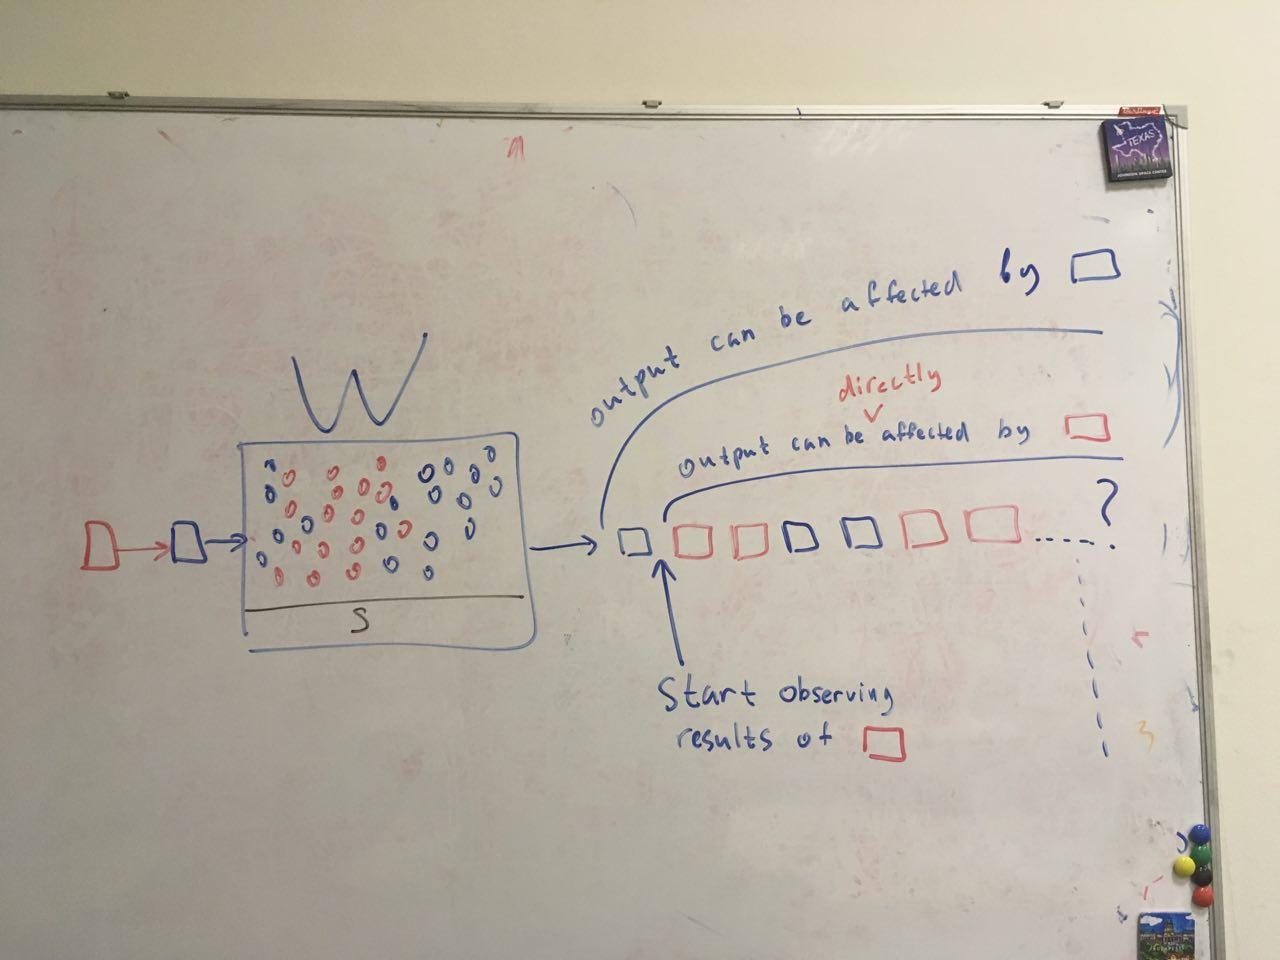
\includegraphics[width=0.48\textwidth]{pics/nullification}
  \caption{The red and blue elements have entered the system. Since that time, it is unclear, when they stop directly affect output elements}
  \label {nullification}
\end{figure}

\begin{definition}{Time quantization}
$t$ is the time of input, output, and nullification:

$t=\begin{cases}
\tau_i:\exists{a_{\tau_i}}, \\
\tau_o:\exists{b_{\tau_o}}, \\
\theta_{a_\tau}:\forall{a_\tau}.
\end{cases}$
\end{definition}

Time quantization allows us to consider only {\em observable} points in time. The time of input and output elements is obviously observed by any system. The mechanisms for tracking nullification vary slightly more. In Storm, a special agent called {\em Acker} is used. In Flink, nullification time is tracked using {\em low watermarks}. In Spark Streaming nullification time for each element in a micro-batch coincides with the time, when the micro-batch is fully processed.

Let $x,a^{1},a^\infty$ be input elements with arbitrary arrival times. $\mathbb{B}_t$ are all output elements by the time $t$:

$\mathbb{B}_t=\bigcup\limits_{i=1}^{t}{b_i}$

Let $p(W_t,\mathbb{B}_t|x,a^{1}...a^\infty)$ be a probability to observe working set $W_t$ and output elements $B_t$ at the time $t$ if input elements are $x,a^{1},a^\infty$. Let us construct three sets:

$X^0=(W_\infty,\mathbb{B}_\infty|p(W_\infty,\mathbb{B}_\infty|a^{1}...a^\infty)\neq{0})$

$X^1=(W_{\theta_{x}},\mathbb{B}_{\theta_{x}}|p(W_{\theta_{x}},\mathbb{B}_{\theta_{x}}|x,a^{1}...a^\infty)\neq{0},\forall{i}:{a^i}\neq{x})$

$X^{*}=(W_{\theta_{x}},\mathbb{B}_{\theta_{x}}|p(W_{\theta_{x}},\mathbb{B}_{\theta_{x}}|x,a^{1}...a^\infty)\neq{0},\\
\exists{i}:{a^i={x}},\exists{y:y\in{W_{\theta_{x}}\setminus{S_{\theta_x}}}\cap{Cl(D)(a^i)}})$

These sets model the {\em observable} output, current elements, and state of a stream processing engine. $X^0$ expresses the case, when element $x$ has not affected the system, so it is a forbidden behavior for at least once and exactly once guarantees. On the other hand, $X^{*}$ defines possible results, after $x$ has been nullified, but $a^i=x$ or its dependencies are in the system. Such behavior can cause inconsistencies in system state due to duplicates and should not be observed if the system provides for at most once or exactly-once. Using these modeled sets now we can define guarantees.

\begin{definition}{At most once}
guarantee is provided by a system iff $\forall{x,a^{1}...a^\infty}:X^{1}\cap{X^{*}}=\emptyset$
\end{definition}

\begin{definition}{At least once}
guarantee is provided by a system iff $\forall{x,a^{1}...a^\infty}:X^{0}\cap{X^{1}}=\emptyset$
\end{definition}

\begin{definition}{Exactly once}
guarantee is provided by a system iff $\forall{x,a^{1}...a^\infty}:X^{1}\cap{X^{*}}=\emptyset \wedge X^{0}\cap{X^{1}}=\emptyset$
\end{definition}

% Now streaming consistency guarantees are defined in terms of correspondences between input, output and the system state. Custom system or user-defined semantics are not considered in this model, e.g., if the system drops all input items, it also can be claimed as supporting exactly-once. Looking from another side, our model formally describes which properties are {\em exactly} supported by state-of-the-art stream processing systems, such as Flink, Storm, Spark Streaming, Samza, MillWheel, etc, so we can discuss its properties in unified terms.

We defined streaming consistency guarantees in terms of the proposed model. This model is suitable for state-of-the-art stream processing systems, such as Flink, Storm, Spark Streaming, Samza, MillWheel, etc, so now we can discuss its properties in unified terms.

\subsection{Implementation properties and notes}

% In this section, we formally define some additional concepts and demonstrate a potential way to reduce latency overhead on consistency guarantees. We mainly consider exactly once, because it is the strongest guarantee, which is extremely valuable in practice.    

\begin{definition}{System failures}
are the time moments, when the system loses its working set. 
\end{definition}

Assume that the system fails at time $\tau_f$. The naive idea for recovering is to simply start processing from the very beginning, i.e., to set $W_{\tau_f+1}=\emptyset$ and to replay the whole input stream. However, storing and replaying the whole input stream is inefficient in terms of both memory and time consuming and can violate consistency guarantees.

\begin{definition}{Snapshot}
at time $\tau_s$ is persistently stored $P_{\tau_s}\subseteq{W_{\tau_s}}$ that is not lost even in case of failure.
\end{definition}

Snapshots allow a system to restart processing since defined points. One approach for taking snapshots is to save (or update) the whole $W_{\tau}$ on each $\tau$. In this case, there is no need to replay input elements, because the system can completely restore computations using only a snapshot. Google MillWheel uses this method for recovering. {\em Strong productions} mechanism allows MillWheel to preserve exactly-once guarantee for the price of persistent updates of $P_\tau=W_\tau$ on each $\tau$~\cite{Akidau:2013:MFS:2536222.2536229}.    

Another approach is to take so-called {\em state snapshots}. This kind of snapshots is considered in practice only within the time quantization $t$. It assumes that $\forall{t_s}:P_{t_s}=S_{t_s}$ and requires replay of input element. Suppose, there is a state snapshot at time $t_s$ and a system fails at time $\tau_f>t_s$. In order to recover processing, system sets $W_{\tau_f+1}=P_{t_s}$ and requests for replay elements $a$ such that $\forall{y\in{Cl(D)(a)}}:y\notin{P_{t_s}}$. The idea of taking snapshots is illustrated in Figure~\ref{snapshotting}.

\begin{definition}{Consistent state snapshot}
$P^{c}_{t_s}=S_{t_s}$ at time $t_s$ is a snapshot such that $\forall{a}\in{Cl^{-1}(D)(P^{c}_{t_s})}:\exists{\theta_a}$.
\end{definition}

\begin{theorem}
A system, that uses state snapshots for recovery, provides for at most once guarantee only if all state snapshots are consistent.  
\end{theorem}

Our notion of consistent state snapshot modifies the classical definition of {\em consistent distributed snapshot} proposed in~\cite{Chandy:1985:DSD:214451.214456} for the case where dependencies between messages exist and input element must be applied to state atomically with its inversed dependencies. This notion is natural for stream processing systems because as it was shown, it is directly connected with streaming consistency guarantees. 

One popular method for taking consistent state snapshot is to artificially reproduce a moment $t_s$, when $\forall{a}\in{Cl^{-1}(D)(S_{t_s})}:\exists{\theta_a}$, and to save obtained $S_{t_s}$. Such approach is adopted in Apache Flink~\cite{Carbone:2017:SMA:3137765.3137777} and Apache Storm~\cite{apache:storm:state}. They achieve consistent state by injecting special elements called {\em checkpoints} into the input elements. Checkpoints go through the same network channels as ordinary elements and push all inverted dependencies of inputs through the system. Each operation in data flow prepares its snapshot independently at the moment of checkpoint arriving. Global snapshot is taken when checkpoint passes through the whole data flow. 

Checkpoints cause latency overhead because they periodically block some inputs of an operation with multiple inputs. This behavior is known as {\em checkpoints alignment}. Consistent state snapshotting can be potentially relaxed if there is a mechanism to retrieve only a consistent part of each operation state at any moment in time. In this case, there is no need to technically reproduce a moment, when it is consistent, in order to obtain it.

Another property that directly affects consistency guarantees is {\em determinism}. Let $a_1...a_\infty$ be ordered in time input elements.

\begin{definition}{Data processing system is {\em deterministic}}
if \\
$\forall{t} \forall{n\geq1} \forall{a_1...a_n}\exists{\mathbb{B}_t={\{b_1...b_m\}}}:\sum\limits_{W_t} p(W_t,\mathbb{B}_t|a_1...a_n)=1$.
\end{definition}

\begin{theorem}
A non-deterministic system provides for at most once guarantee only if $\forall{b_{t_o}}:\exists{P^{c}_{t_o}} \wedge \forall{a\in{Cl^{-1}(b_{t_o})}},\theta_a=t_o$.  
\end{theorem}

Hence, non-deterministic systems that use state snapshots must atomically output elements and take a consistent snapshot that contains their inverted dependencies in order to achieve exactly once. In practice, it means that the lower bound of latency in the worst case in such systems is the time between snapshotting together with the duration of taking a snapshot. There is a trade-off between latency and the frequency of taking snapshots because too frequent snapshotting can cause high extra load, while rare snapshots lead to high latency. We can observe such behavior in all stream processing systems that provide for exactly once and use state snapshots, e.g., in Flink atomicity between state snapshotting and elements releasing is preserved using the modification of 2PC protocol. On the other hand, if a system is deterministic, atomicity between output and snapshotting is not necessary, because in case of replay system releases exactly the same output, that can be somehow deduplicated.

\section {Discussion}
The roadmap of approaches for achieving exactly-once is shown in Figure~\ref{roadmap}. White bricks show the paths, which are used by state-of-the-art stream processing systems. Unfortunately, all these approaches have a high latency overhead. Working set snapshotting requires frequent blocking accesses to persistent storage. Atomic snapshotting and releasing make latency dependent on the time between snapshots. Micro-batching approaches experience high latency, because of the buffering on input.    

\begin{figure*}[htbp]
  \centering
  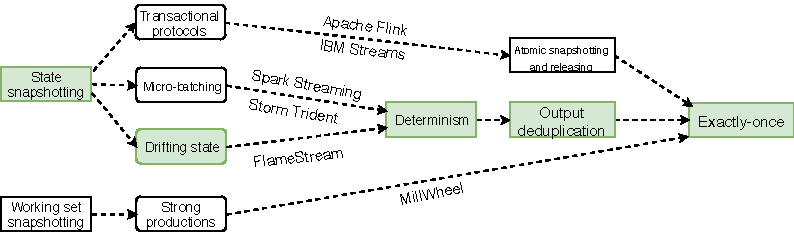
\includegraphics[width=0.97\textwidth]{pics/roadmap}
  \caption{The roadmap of approaches for achieving exactly-once guarantee. Green elements indicate the path for our approach}
  \label {roadmap}
\end{figure*} 

To the best of our knowledge, only micro-batching systems apply determinism for achieving exactly-once. It is commonly assumed that it is extremely hard to make a stream processing system deterministic without high latency overhead. One reason behind this fact is that in general, Spark Streaming provides higher latency than pure streaming engines, e.g., Flink~\cite{karimov2018benchmarking}. However, in~\cite{we2018adbis} there was proposed a model called {\em drifting state} that allows achieving both determinism and low latency. Therefore, the open questions are: is it more efficient in practice to handle non-determinism by atomic snapshotting and releasing than to maintain a fair determinism in order to get exactly once? Can the green path provide lower latency than the most efficient white?

\section {Drifting state model}
%%% fs-state-model - Model

\label {fs-model-section}

In this section, we outline the model of our system. We focus on the core concepts and definitions to introduce the necessary preliminaries for consistency preserving mechanisms. \FlameStream\ model has much in common with other stream processing systems but has several vital differences that enables the opportunity for efficient implementation of consistency guarantees. Among them are reduced set of operations, strict ordering and cyclic graphs.

\subsection{Data flow}
The basic data flow abstraction is a {\it stream}. The stream is represented by an infinite heterogeneous sequence of data items. Data item is a {\it payload} and a {\it meta-information} associated with it. 

\[DataItem := (Payload, Meta)\]

The payload is an arbitrary user-provided data. Meta is structured system-assigned information. The primary purpose of the meta-information is to impose the total order on data items. Part of meta information is an application time - logical time, provided by data-producer, that is used for initial ordering.

Inside stream, data items can be dropped or transformed into the new data items.

\subsection{Boundaries}
Data producers are external to our system. {\em Front} is a component that acts as a mediator between them and a computational pipeline.

At the end of a pipeline, there is a {\em barrier} that prepares results to be consumed by user. The main role of a barrier is to filter out possible duplicates or invalid results. Another function is to carry out an output protocol between system and data consumers, which is an essential part of providing exactly-once semantics.

\subsection{Computational flow}
The stream between front and barrier is handled by a user-provided directed data flow graph. Each node of the graph represents a single operation parameterized by user-defined business-logic. An operation can have multiple inputs and outputs. Edges indicate the order of these operations. Data items are processed one-by-one in a "streaming" manner. Our model allows cycles in the graph while data flow graphs are commonly assumed to be acyclic (DAGs) 
~\cite{Zaharia:2016:ASU:3013530.2934664, Carbone:2017:SMA:3137765.3137777}.

\subsection{Physical deployment and partitioning}
In order to perform actual computations, data flow graph is distributed among computational units. Each unit runs a process called {\it worker}, and each of the workers executes complete data flow graph. The range of 32-bit signed integer is divided into the fixed number of non-intersecting {\it hash units}. Each worker can be responsible for one or many hash units. Hash units are used further for partitioning and state saving. The number of hash-units per worker is a user-defined parameter, and it must be set before the start of computations. 

Each operation input has a user-provided hash function called {\it balancing function}. This function is applied to the payload of data items and determines partitioning before each operation. After that, the data items are sent to the worker, which is responsible for the associated hash unit. Therefore, load balancing explicitly depends on the user-defined balancing functions. It allows the developer to determine optimal balancing which requires the knowledge of the payload distribution. The system optimizes the hash ranges assignment according to the processing statistics. 

\subsection{Ordering assumptions}
The system enforces a total order on data items. Ordering is preserved when an item is traveling through the operations. More precisely, the order of output items is the same as the order of corresponding input items. If more than one item is generated, they are inserted in output stream sequentially. Moreover, the output follows corresponding input but precedes the next item. This rule is vital for cycle processing. Without diving into details, it should be noted that the order of items is maintained across different fronts.

The concept of ordering is shown in Figure~\ref{ordering}. Data item with payload $1'$ is the derivative of the item with payload $1$, according to operation $F$. The same is for items with payloads $2'$ and $2$. After union operation, the order between $1$ and $2$ is preserved. Furthermore, $1'$ follows $1$, and $2'$ follows $2$.  
\begin{figure}[htbp]
  \centering
  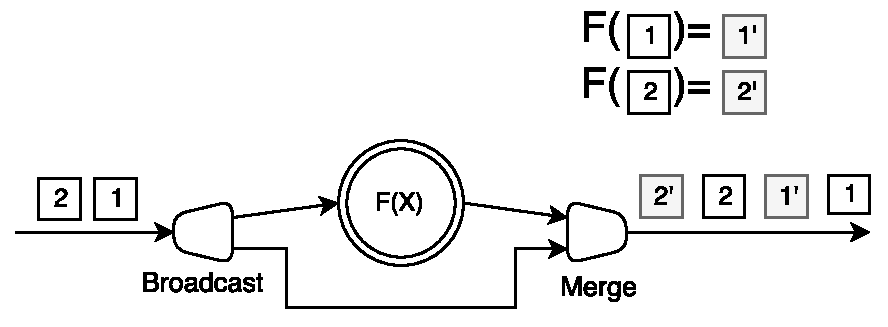
\includegraphics[width=0.48\textwidth]{pics/ordering}
  \caption{The concept of ordering model}
  \label {ordering}
\end{figure}

We assume that input items of the operations are strictly ordered.

\subsection{Supported operations}
The list of available operations includes:

{\bf Map} applies a user-defined function to the payload of an input item. This function returns a sequence of data items with transformed payloads. An output sequence can be empty.

{\bf Broadcast} replicates an input item to the specified number of operations.

{\bf Merge} operation is initialized with the specified number of input nodes. It sends all incoming data to the output.

{\bf Grouping} has a {\it window size} parameter. Grouping stores input items into distinct buckets by the value of the input balancing function applied to the payload. When the next item arrives at the grouping, it is appended to the corresponding bucket. Each time the grouping outputs window-sized {\it tuple item}, which consists of the most recent (in terms of the meta-information) items of this bucket. If the size of the bucket is less than the window, all items of the bucket are taken. Grouping is the only operation that has a state.

The following example illustrates the semantics of the operation. The grouping accepts items with payload represented as natural numbers: 1,2,3, etc. The hash function returns 1 if the number is even and 0 otherwise. If the window is set to 3, the output elements are:

\[(1), (2), (1|3), (2|4), (1|3|5), (2|4|6), (3|5|7), (4|6|8)...\]

There are two important properties of the grouping operation: the output tuples are ordered by their last elements, the results among items with different values of a hash function are independent.

\subsection{Stateful transformations}
The given set of operations jointly with cyclic execution graphs is enough to implement any stateful operation, i.e., reduce in terms of MapReduce model. The scheme of such transformations is out of the scope of this paper. It is deeply detailed in~\cite{we2018seim}.

\subsection{Implementation notes}

As it was defined previously, in our model only the grouping operation maintains a state and the state depends on the order of incoming items. Therefore, to achieve deterministic processing, there is a need to enforce the right order. However, conservative methods for the order enforcing are based on buffering~\cite{Li:2008:OPN:1453856.1453890} and can imply high latency overhead. The main difficulty here is that items can be easily reordered within stream processing systems because of asynchrony and the possible existence of multiple paths between two nodes. 

In~\cite{we2018seim} an optimistic approach to handle out-of-order items was introduced. The key idea behind it is that grouping can produce invalid results, but they must be filtered out at the barrier. Therefore, there is a need to buffer output items at the barrier before it is ensured that there are no invalid invalid in-flight items and they cannot be generated. It is convenient to release items by global times.

To track the global time of in-flight items we adopt an idea of {\it acker task} inspired by Apache Storm~\cite{apache:storm}. Acker tracks data items using a checksum hash. When the item is sent or received by an operation, its global time and checksum are sent to the acker. This message is called {\it ack}. Acker groups acks by a global time into the structure called {\it ack table}. Once acker receives an ack message with global time {\it GT} and {\it XOR} it updates {\it GT} entry in the table by xoring {\it XOR} with the current value. When an item is sent and later received by the next operation, xoring corresponding {\it XOR}s would yield zero.

Acks are overlapped to nullify table's entry only when an item arrives at the barrier. That is, ack for receive is sent only after both processing and the ack sending for the transformed item, as illustrated in Figure~\ref{acker}. Different shapes of items mean different payloads. The ack for the sending of the triangular element is sent before the rectangular one. We expect the channel between the acker and each operation to be FIFO, so ack for the triangular item would be xored before the rectangular. So the two equal values are separated by distinct one. This technique guarantees that the {\it XOR} for some global time is equal to zero only if there are no in-flight elements with such global time.

\begin{figure}[htbp]
  \centering
  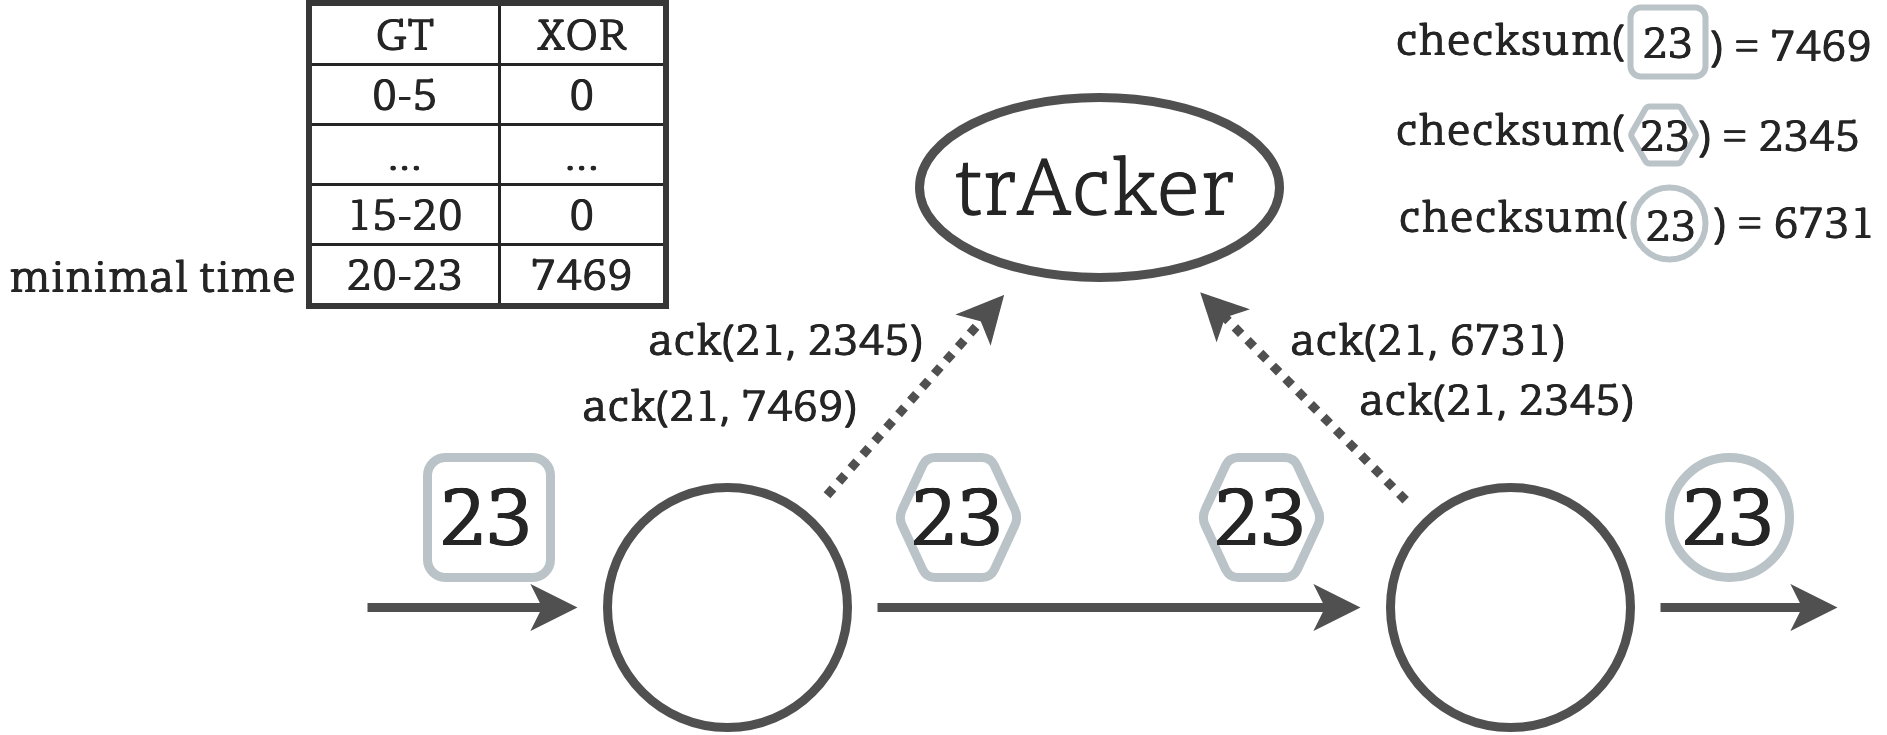
\includegraphics[scale=0.58]{pics/acker}
  \caption{The example of tracking minimal time using acker}
  \label {acker}
\end{figure}

The minimal time within a stream is the minimal global time with non-zero {\it XOR}. On minimal time changes, acker broadcasts new minimal time to the barrier and operations. Minimal time notifications plays the same role as {\em low-watermarks} in OOP architecture~\cite{Li:2008:OPN:1453856.1453890}. Therefore, the barrier can release elements with global time {\it GT} once it received notification from acker that the minimal time within the stream is greater than {\it GT}.

The important implication of ack-table structure is that items that was generated by a single input event become ready for releasing at the same moment.

To ensure that no fronts can generate item with the specific timestamp, each front periodically sends to acker special message called {\it report}, which promises that front will not generate items with a timestamp lower than the reported. The value in the ack table can become zero only after the corresponding report arrives.

It must be noted that acker can play the role of worker's coordinator because it observes the progress of the whole system. This property is used further in the implementation of mechanisms for fault tolerance. 

\FlameStream\ is implemented in Java, using Akka framework for messaging and applies Apache ZooKeeper as a {\it cluster state manager}. The usage of ZooKeeper mitigates the need for the dedicated master node. Some persistent storage is needed for reliable state saving. An overview of the \FlameStream\ system model and architecture is shown in Figure~\ref{arch}.

\begin{figure*}[htbp]
  \centering
  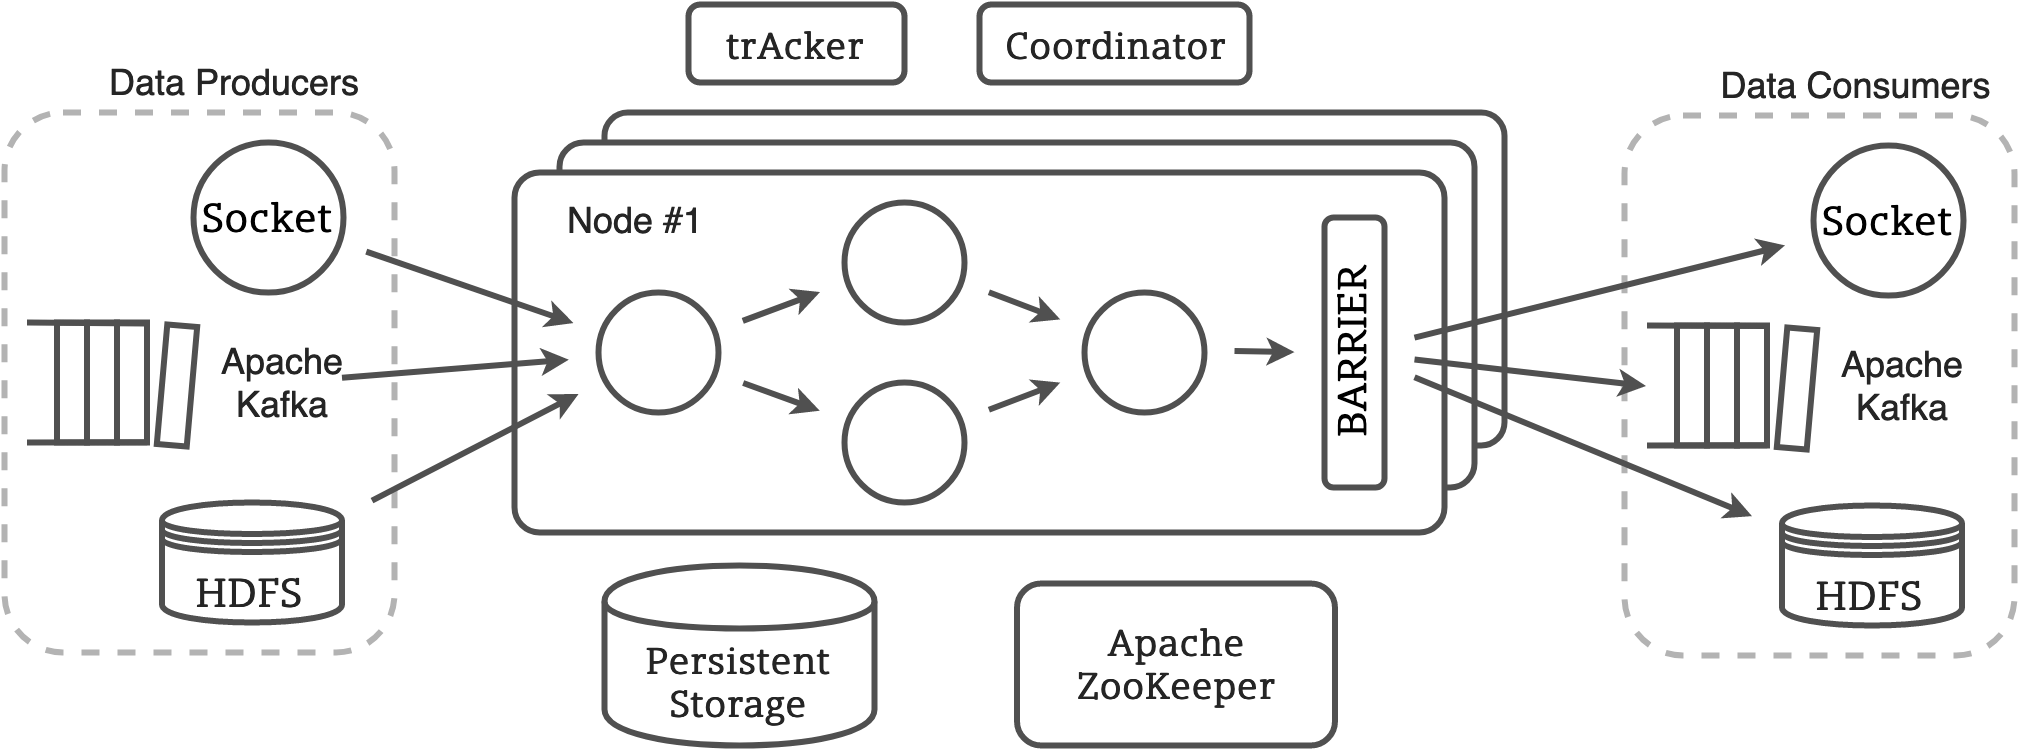
\includegraphics[scale=0.58]{pics/arch}
  \caption{The overview of FlameStream physical architecture}
  \label {arch}
\end{figure*}

\subsection{Consistency guarantees}
There are three main types of consistency guarantees relating to stream processing. {\it At most once} semantics states that each input event is processed once or not processed at all. {\it At least once} guarantees that each input item is processed, but possibly multiple times, that can lead to result duplication or state inconsistency. {\it Exactly once} semantics guarantee that each input event is processed exactly one time. 

The properties of the proposed model provide several useful features for achieving exactly-once semantics. The total order directly leads to the property of determinism, while optimistic approach for handling out-of-order items allows to enforce it with low overhead. In turn, as it was mentioned above, determinism is a convenient base for system-wide idempotence. The roadmap of our approach is shown in Figure~\ref{roadmap}. The exact techniques to achieve exactly-once are detailed in the next section. 


\section{Implementation}
%%% fs-state-consistency - Fault tolerance

\label {fs-consistency-section}

In the previous section, we demonstrated how state-of-the-art stream processing systems handle non-deterministic behavior in order to achieve~ exactly-once. All these systems make state recoverable before output elements which depend on this state are released. As we demonstrate further, such behavior can significantly increase the processing latency of individual elements.

The condition from the Theorem~\ref{necessary_conditions} can be relaxed for a deterministic system because determinism guarantees order enforcement before non-commutative operations. If a system is deterministic, it is possible to recompute states of non-commutative operations consistently. Hence, such a system can release an output element before a snapshot is taken because it can reproduce the same state in case of failure. It means that even if elements are divided into the epochs like in Apache Flink, and a snapshot is taken once per epoch, ready-to-release output elements should not wait until the epoch is committed in order to be delivered. The limitation of this approach is that only deterministic operations (e.g. without the usage of random values) are allowed in a data flow.

To combine the determinism with  exactly-once we need to design protocols for recovery function $F$ and saving data needed for correct restoring. In this section, we describe protocols for exactly-once enforcement on top of a lightweight deterministic model for distributed stream processing called {\em drifting state}~\cite{we2018adbis}. This model is implemented in~\FlameStream\ processing system~\cite{we2018beyondmr}.

In~\FlameStream\, computations are deterministic due to a (speculative) maintenance of a pre-defined total order on elements before each order-sensitive operation. The order can be defined using various methods~\cite{we2018seim}, and we assume that $\forall x_1,x_2\in \Gamma, \exists t(x): x_1 < x_2 \Longleftrightarrow t(x_1) < t(x_2)$. In order to achieve exactly-once on top of a deterministic stream processing system we propose the following way:
\begin{itemize}
    \item Periodically save (take a snapshot of) operation states
    \item Consistently restore these states and replay missed input elements in case of failure
    \item Ensure that output elements which have been already released will not be duplicated after recovery and input reprocessing
\end{itemize}

We do not enforce a strict architecture of the system, but assume that there are several functional agents:
\begin{itemize}
    \item Coordinator manages snapshotting and recovery.
    \item Cluster state manager is used to keep service information for recovery.
    \item Persistent storage is needed for reliable storing of state snapshots. In case of failures, the state snapshot is recovered from persistent storage.
    \item Data producer that can replay some set of previous input elements with the same $t(a)$.
    \item Data consumer that is responsible for output elements receiving. The exact requirements for data consumer are detailed further in this section.
    \item Node is an executor of user-defined operations. The computation can be balanced through the distribution of data elements among nodes. Each Node has a {\em barrier} that delivers output elements to the end-user.
\end{itemize}

The implementation of this architecture in~\FlameStream\ processing engine is demonstrated in Figure~\ref{arch}. Apache ZooKeeper is used for cluster state management. As persistent storage, one can use a distributed file system or database (e.g., HDFS, S3, MongoDB, GFS, HBase, etc.). Data producers may vary as well: the role of $t(a)$ can be played by any monotonic sequence, e.g., offsets in Kafka.

\subsection{Snapshotting}

\subsubsection{Operation states}

In order to periodically save operation states, there is a need to determine which input elements affect them. 
 We have to trace reversed dependencies: for each state element $s$ we desire to determine such input elements $\{a_i\}$ that $\forall i, s \in Cl_D^{-1}(a_i)$. Otherwise, it may be unclear, which input elements must be reprocessed during recovery. In Apache Flink, it is implemented through specific streaming elements which play the role of notifications that a determined set of input elements have been processed. In~\FlameStream\ this mechanism is implemented using a modification of {\em Acker} agent from Apache Storm~\cite{apache:storm}. 

Assuming that the mechanism for detection of which input elements influence states is implemented, the protocol of state snapshotting for {\em Coordinator} and {\em nodes} is the following:

\begin{itemize}
    \item Coordinator decides that snapshot should be taken and enables a mechanism to detect which input elements have been processed since the previous snapshot.
    \item On the notification, nodes asynchronously make operation states recoverable and send to Coordinator the acceptance message.
    \item When the Coordinator receives all acceptance messages, it saves the information about which input elements belong to this snapshot and other service information about the snapshot. In general, it is sufficient to save only $t(a)$ of the last input element that affects the snapshot.
\end{itemize}

It is worth to note that the proposed protocol is similar to the transactional (variation of 2PC) state snapshotting protocol used in Flink~\cite{Carbone:2017:SMA:3137765.3137777}. The critical difference is that in our method, output releasing agents (barriers) do not take part in a distributed transaction, because in a deterministic system there is no need to wait until the snapshot is taken in order to release output elements consistently. The scheme of the protocol used in Apache Flink is shown in Figure~\ref{protocol_flink}. As it is demonstrated, output elements delivery (stage 4) is allowed only after commit (stage 3). Modified state snapshotting protocol for a deterministic system is demonstrated in Figure~\ref{protocol_fs}. One can note that elements delivery is independent of the snapshotting protocol. This difference determines the significant latency decrease that is demonstrated further in experiments.

\begin{figure}[htbp]
  \centering
  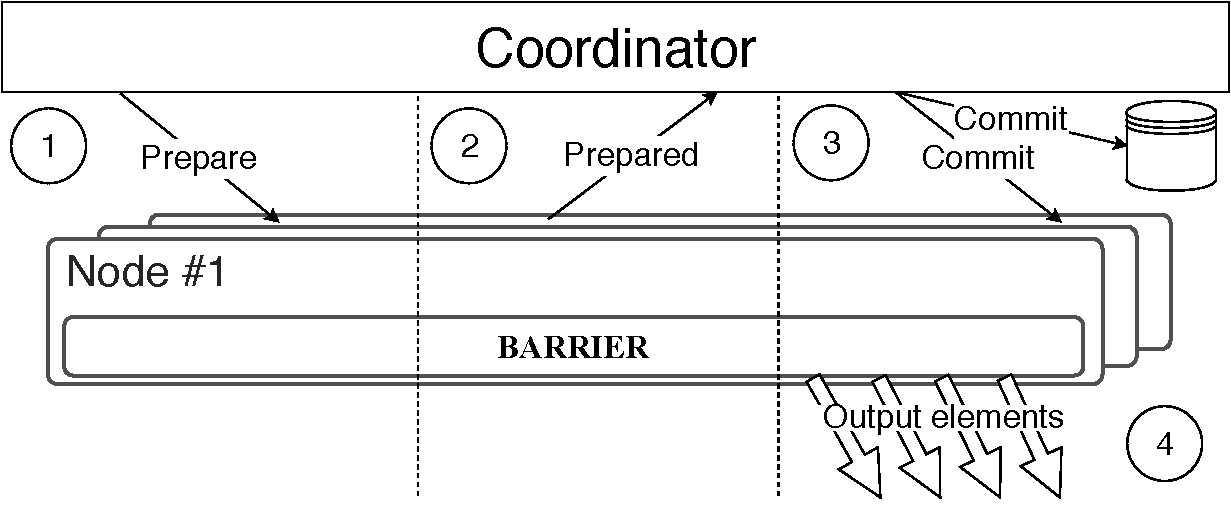
\includegraphics[width=0.42\textwidth]{pics/protocol-flink}
  \caption{State snapshotting protocol in Apache Flink}
  \label{protocol_flink}
\end{figure}

\begin{figure}[htbp]
  \centering
  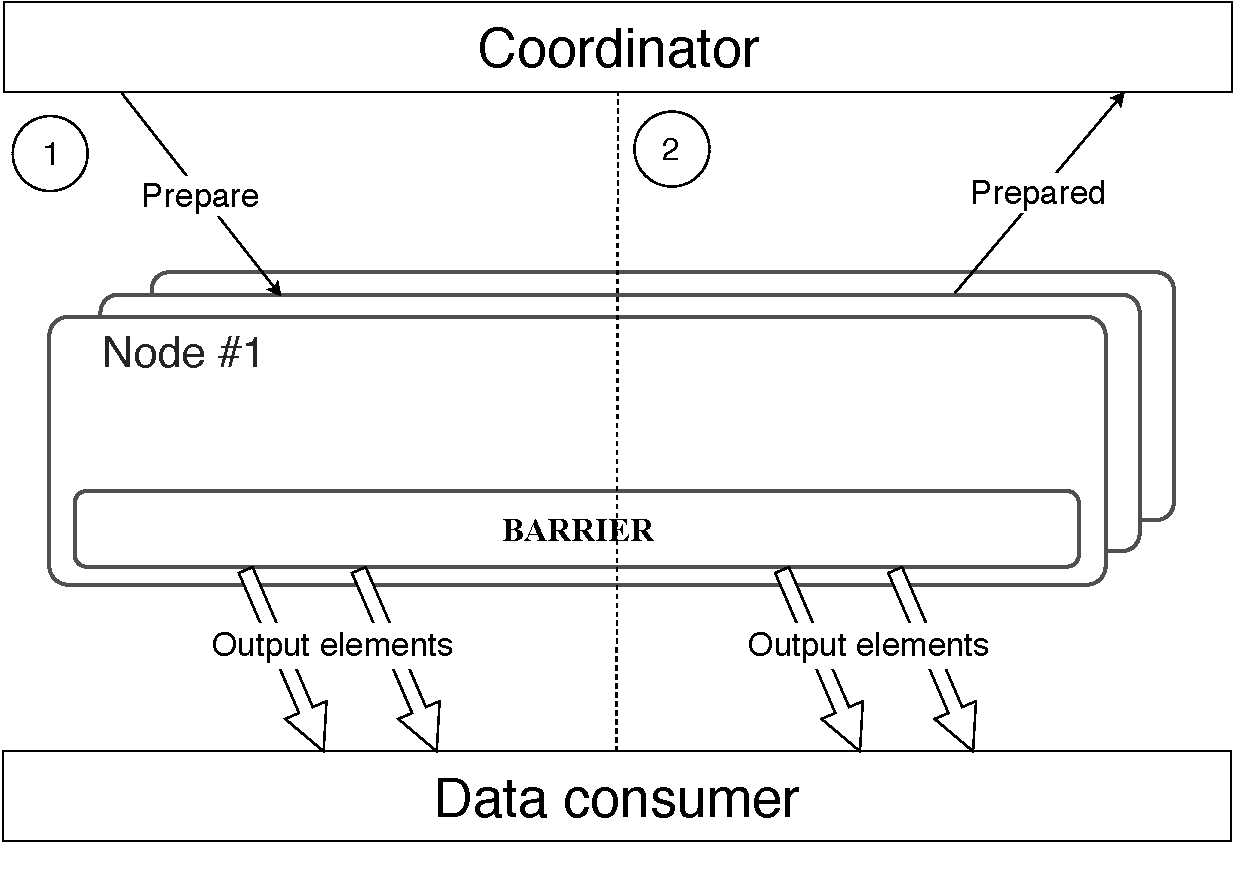
\includegraphics[width=0.42\textwidth]{pics/protocol-fs}
  \caption{State snapshotting protocol in a deterministic system}
  \label{protocol_fs}
\end{figure}

\subsubsection{Last output element}

In order to preserve the deterministic outcome, the Barrier must release output items with monotonically increasing $t(x)$. Hence, the Barrier can filter out any items with $t(x)$ less than or equal to the $t(x)$ of the last released item $t_{last}$ in order to preserve exactly-once after recovery. To implement this mechanism, there is a need to deliver output items and update $t_{last}$ atomically. To solve this problem, we require the following output protocol between a {\em barrier} and a {\em data consumer}: 

\begin{itemize}
    \item On each output delivery, Barrier sends a bundle to the data consumer. This bundle contains an output item and $t_{last}$. The Consumer must acknowledge that it received the bundle.
    \item Barrier does not send new output bundle until the previous one is not acknowledged.
    \item Consumer must return last received bundle on Barrier's request.
\end{itemize}

This protocol guarantees that $t_{last}$ and released items are always consistent with each other. It implies that the Barrier can request the last released bundle and fetch $t_{last}$ after recovery to avoid duplicates, which can be generated during input elements reprocessing.

Thus, on the one hand, we delegate the part of the basic functionality to data consumers. On the other hand, the requirement for a data consumer is not so strong and can be naturally satisfied by real-world consumers (HDFS, Kafka, databases, etc.). 

\subsection{Recovery}

Typically, distributed systems take into consideration the following types of failures:
\begin{itemize}
    \item Packet loss
    \item Node failure
    \item Network partitioning
\end{itemize}

Network partitioning is the particular case of failure because in this case, computations cannot be restarted. We believe that in this case, stream processing does not make sense. To the best of our knowledge, there are no open-source stream processing systems that tolerate network partitioning.

Failure detection can be implemented in different ways~\cite{hayashibara2002failure}, which are out of the scope of this paper. In~\FlameStream\ it is implemented using {\em Acker}~\cite{we2018adbis}. In the case of packet loss or node failure, a failure detector mechanism can enforce the Coordinator to begin computations restart from the last successful snapshot. Restart protocol includes the following steps:

\begin{itemize}
    \item Coordinator broadcasts a notification to begin the recovery process.
    \item Operations receive these notifications and fetch their states from state storage. After that, they send an acknowledgment that they are ready for Processing to the Coordinator.
    \item Barriers request the last released bundle from data consumers and send acknowledgments that they are ready for Processing to the Coordinator.
    \item When the Coordinator receives all acknowledgments from groupings and barriers, it requests data producer to replay starting from the $t(a)$ of the last snapshot.
\end{itemize}

The proposed protocol guarantees the following properties that allow preserving~ exactly-once:

\begin{itemize}
    \item Processing does not restart until all operations obtain consistent states. The consistency of these states is guaranteed by the state snapshotting protocol. Therefore, the elements are not lost.
    \item Duplicates are not produced because, at the moment when Processing is restarted, it is ensured that Barrier has obtained the last released $t(x)$ and can filter out extra items.
\end{itemize}

\section {Experiments}
%%% fs-state-experiments - Experiments

\label {fs-experiments-seciton}

\subsection{Setup}
The series of experiments were performed in order to analyze the overall performance of the system's prototype. We apply building an inverted index as a stream processing task for the evaluation. Building inverted index is implemented as a MapReduce transformation which is shown in Figure~\ref{index}: 

\begin{itemize}
    \item Map phase includes conversion of input documents into the key-value pairs {\it (word; word positions within the page)}
    \item Reduce phase consists of combining word positions for the corresponding word into the single index structure 
\end{itemize}

Reduce phase outputs the change records of the inverted index structure, to make this algorithm suitable for stream processing systems. It implies that each input page triggers the output of the corresponding change records of the full index. In \FlameStream\ this algorithm is implemented as the typical conversion of MapReduce transformation, which is shown in~\cite{hiddenSeim}.

\begin{figure}[htbp]
  \centering
  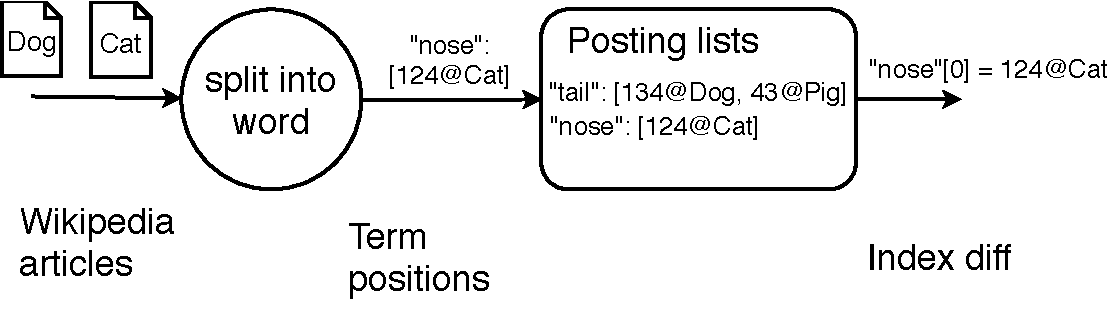
\includegraphics[width=0.50\textwidth]{pics/index}
  \caption{The inverted index pipeline}
  \label {index}
\end{figure}

We chose the task of building an inverted index because it satisfies the following properties:

\begin{itemize}
    \item The computational pipeline of the task contains network shuffle that can violate the ordering constraints. Therefore, this task is able to estimate the performance of the proposed deterministic model fairly
    \item Consistency guarantees are strongly required because the inconsistent index does not make sense for many applications
    \item The workload is unbalanced due to Zipf's law
\end{itemize}

Notably, building an inverted index in a streaming manner can be the halfway task between the generation of documents and consuming index updates by search infrastructure. In the real world, this scenario can be found in freshness-aware systems, e.g., news processing engines.

By the notion of {\it latency} we assume the time between two events: 

\begin{enumerate}
    \item Input page is taken into the stream
    \item All the change records for the page leave the stream
\end{enumerate}

Our experiments were performed on the cluster of 10 Amazon EC2 micro instances with 1GB RAM and 1 core CPU. We used Wikipedia articles as a dataset. Documents per second input rate is 50. RocksDB~\cite{rocksdb} is used as a storage for the state. The role of data producer and data consumer is played by a custom server application that sends and receives data through socket and measures the latency.

\subsection{Overhead and recovery}
The performance of the proposed deterministic model within the same stream processing task is deeply analyzed in~\cite{hiddenSeim}. In this paper, we aim to evaluate the overhead on providing consistency guarantees and the time needed for the full recovery.

Figures~\ref{comparison50}, ~\ref{comparison500}, and ~\ref{comparison1000} shows the latencies of \FlameStream\ within distinct times between checkpoints, and at most once, at least once, and exactly once consistency semantics. As expected, the overhead on at least once and exactly once semantics is low (less than 10 ms), and it does not depend on the time between checkpoints. Slight overhead can be explained by the fact that asynchronous state snapshotting is executed on single-core nodes. The time between checkpoints does not influence latency because barrier flushing and state snapshotting mechanisms are independent in our model. The latencies under at least once and exactly once semantics are the same because the only difference between them regarding our model is in contract with data consumer.

System's behavior in case of failures and recoveries is demonstrated in Figure~\ref{recovery}. It is shown that the system can perform recovery processes in an adequate time. Existing latency spikes are caused by the replay process, JVM restart, etc.

\begin{figure}[htbp]
  \centering
  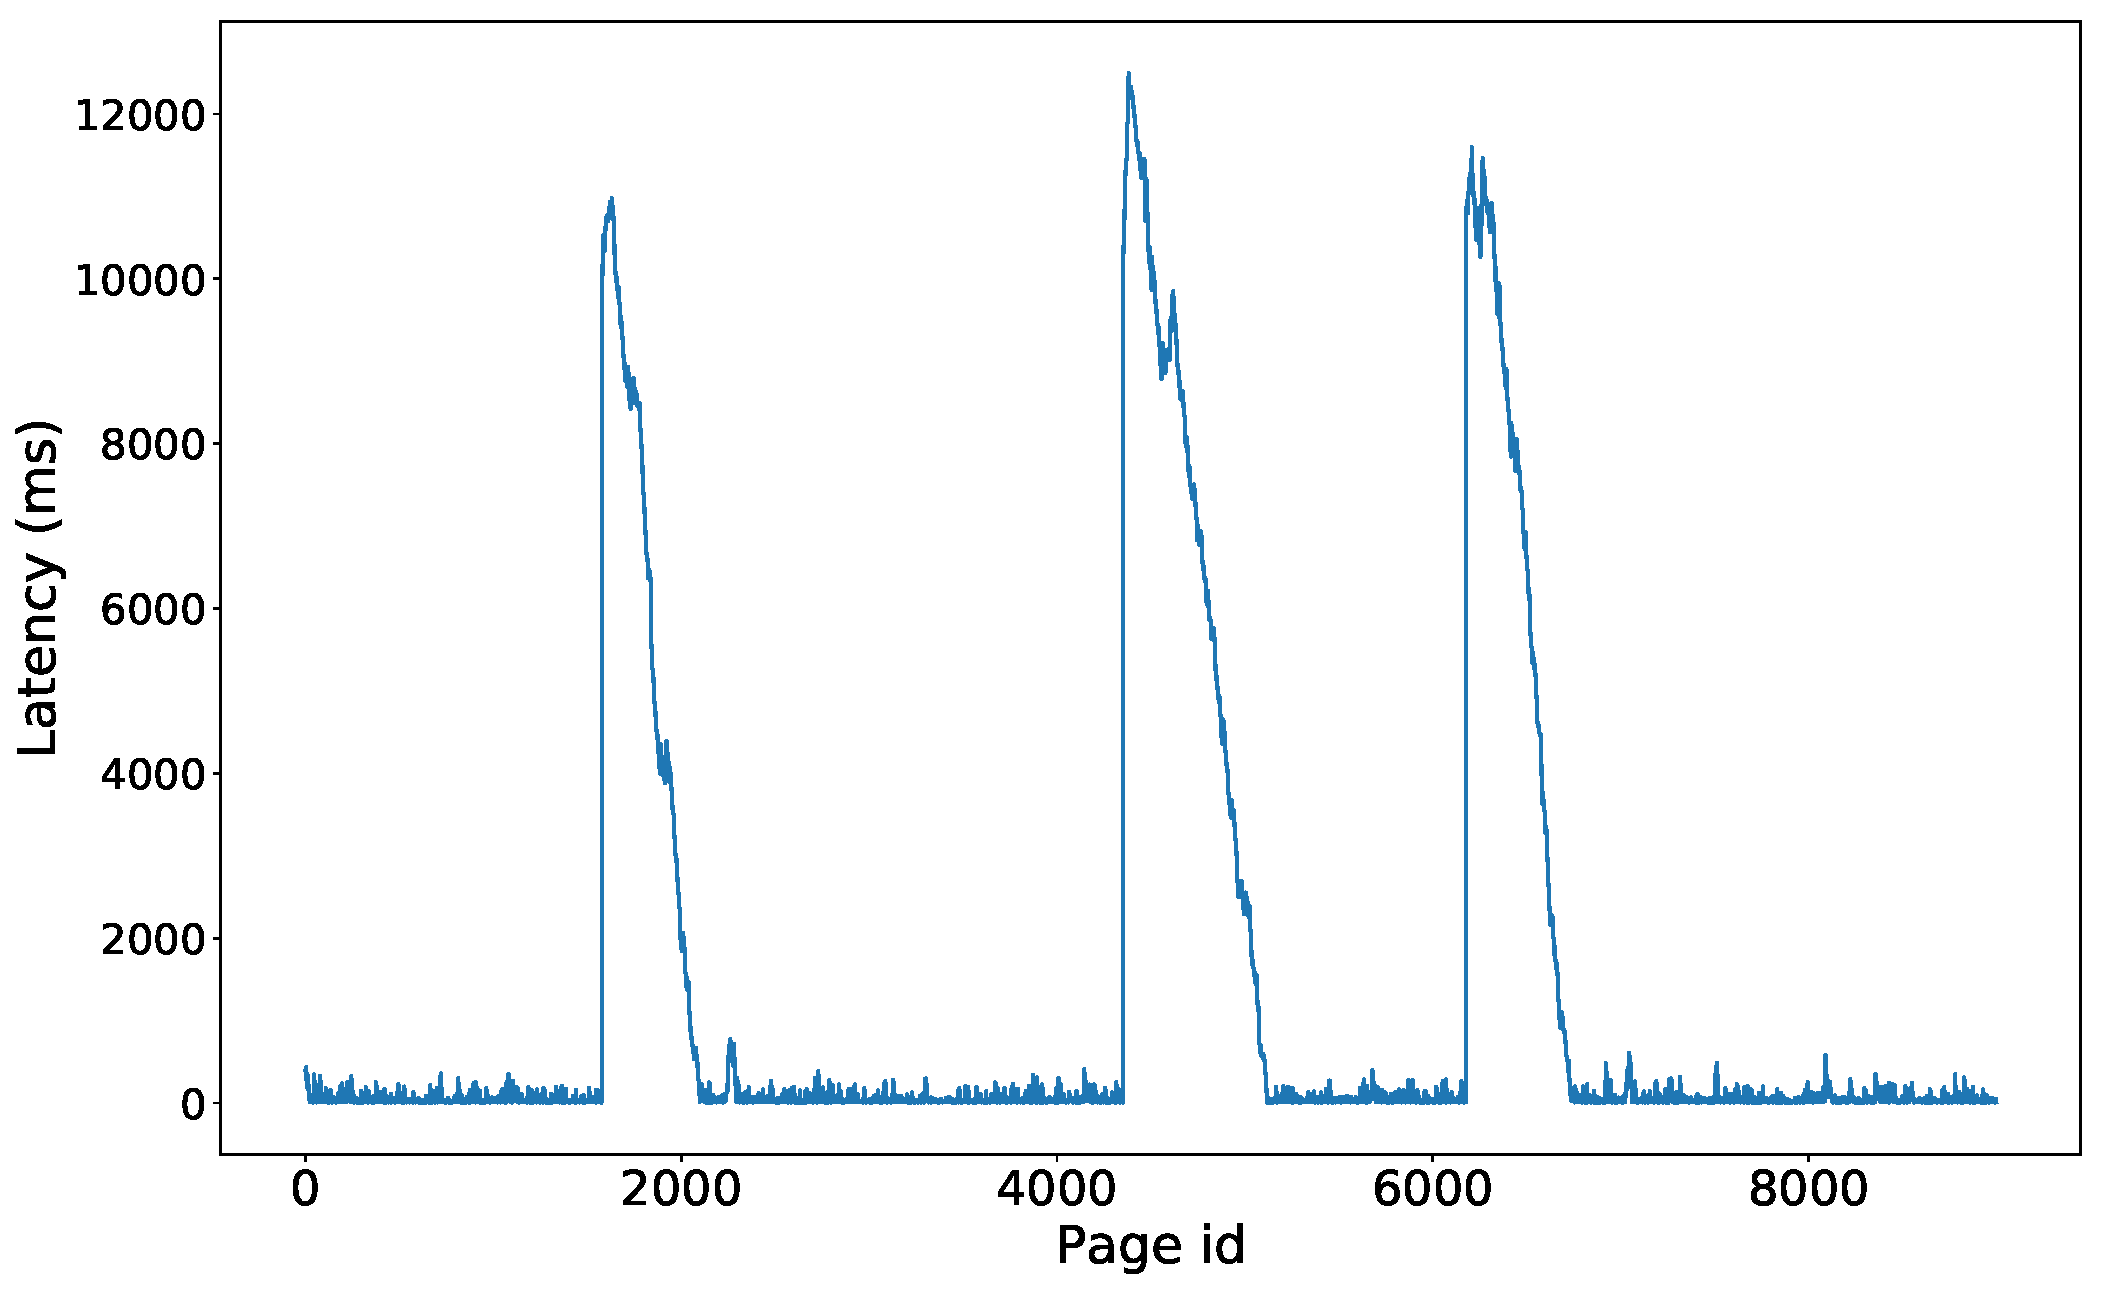
\includegraphics[width=0.48\textwidth]{pics/blink}
  \caption{The latencies of \FlameStream\ during three failures and recoveries}
  \label {recovery}
\end{figure}

\subsection{Comparison against Apache Flink}
One of the most important goals of the experiments is the performance comparison with an industrial solution regarding latency. Apache Flink has been chosen for evaluation because it is a state-of-the-art stream processing system that provides similar functionality and achieves low latency in the real-world scenarios~\cite{S7530084}. 

For Apache Flink, the algorithm for building the inverted index is adopted by the usage of {\it FlatMapFunction} for map step and stateful {\it RichMapFunction} for reduce step and for producing the change records. Order enforcing before reduce is implemented using custom {\it ProcessFunction} that buffers all input until corresponding low watermark is received. Watermarks are sent after each document. The network buffer timeout is set to 0 to minimize latency. Custom {\it TwoPhaseCommitSinkFunction} that buffers output items in memory until a transaction is committed is used for experiments that require exactly-once semantics. 

{\it FsStateBackend} with the local file system is used for storing the state, because {\it RocksDBStateBackend} requires saving state to RocksDB on each update that leads to additional overhead. {\it FsStateBackend} stores state on the disk only on checkpoints and do not provide an additional overhead against RocksDB storage in \FlameStream, so it is fairer to use it rather than {\it RocksDBStateBackend} for comparison purposes.

In this paper, we compare $50^{th}$, $75^{th}$, $95^{th}$, and $99^{th}$ percentile of distributions, which clearly represent the performance from the perspective of the users' experience.

Figures~\ref{comparison50}, ~\ref{comparison500}, and ~\ref{comparison1000} demonstrates the comparison of latencies between \FlameStream\ and Flink within distinct times between checkpoints, and different consistency semantics. At the initial point, \FlameStream\ provides lower latency for at most once semantics. Such behavior is explained by the features of the optimistic approach for handling out-of-order items and is investigated in details in~\cite{hiddenSeim}. The latencies of both \FlameStream\ and Flink are slightly higher under at least once semantics. As it was mentioned above, it can be explained by the single-core configuration of the nodes. For at most once and at least once semantics, the latencies of \FlameStream\ and Flink do not vary a lot because both systems do not buffer output items for a long time before releasing. However, for exactly once semantics, Flink's latency is dramatically higher, and it directly depends on the time between checkpoints. Nevertheless, such behavior is expected, because unlike \FlameStream, Flink needs to take state snapshot and release output items within a single transaction to preserve exactly once semantics. As it was discussed above, it is the consequence of the lack of determinism in the computational model. Therefore, output items cannot be released until the transaction is committed and this fact significantly increases the latency. 

\begin{figure}[htbp]
  \centering
  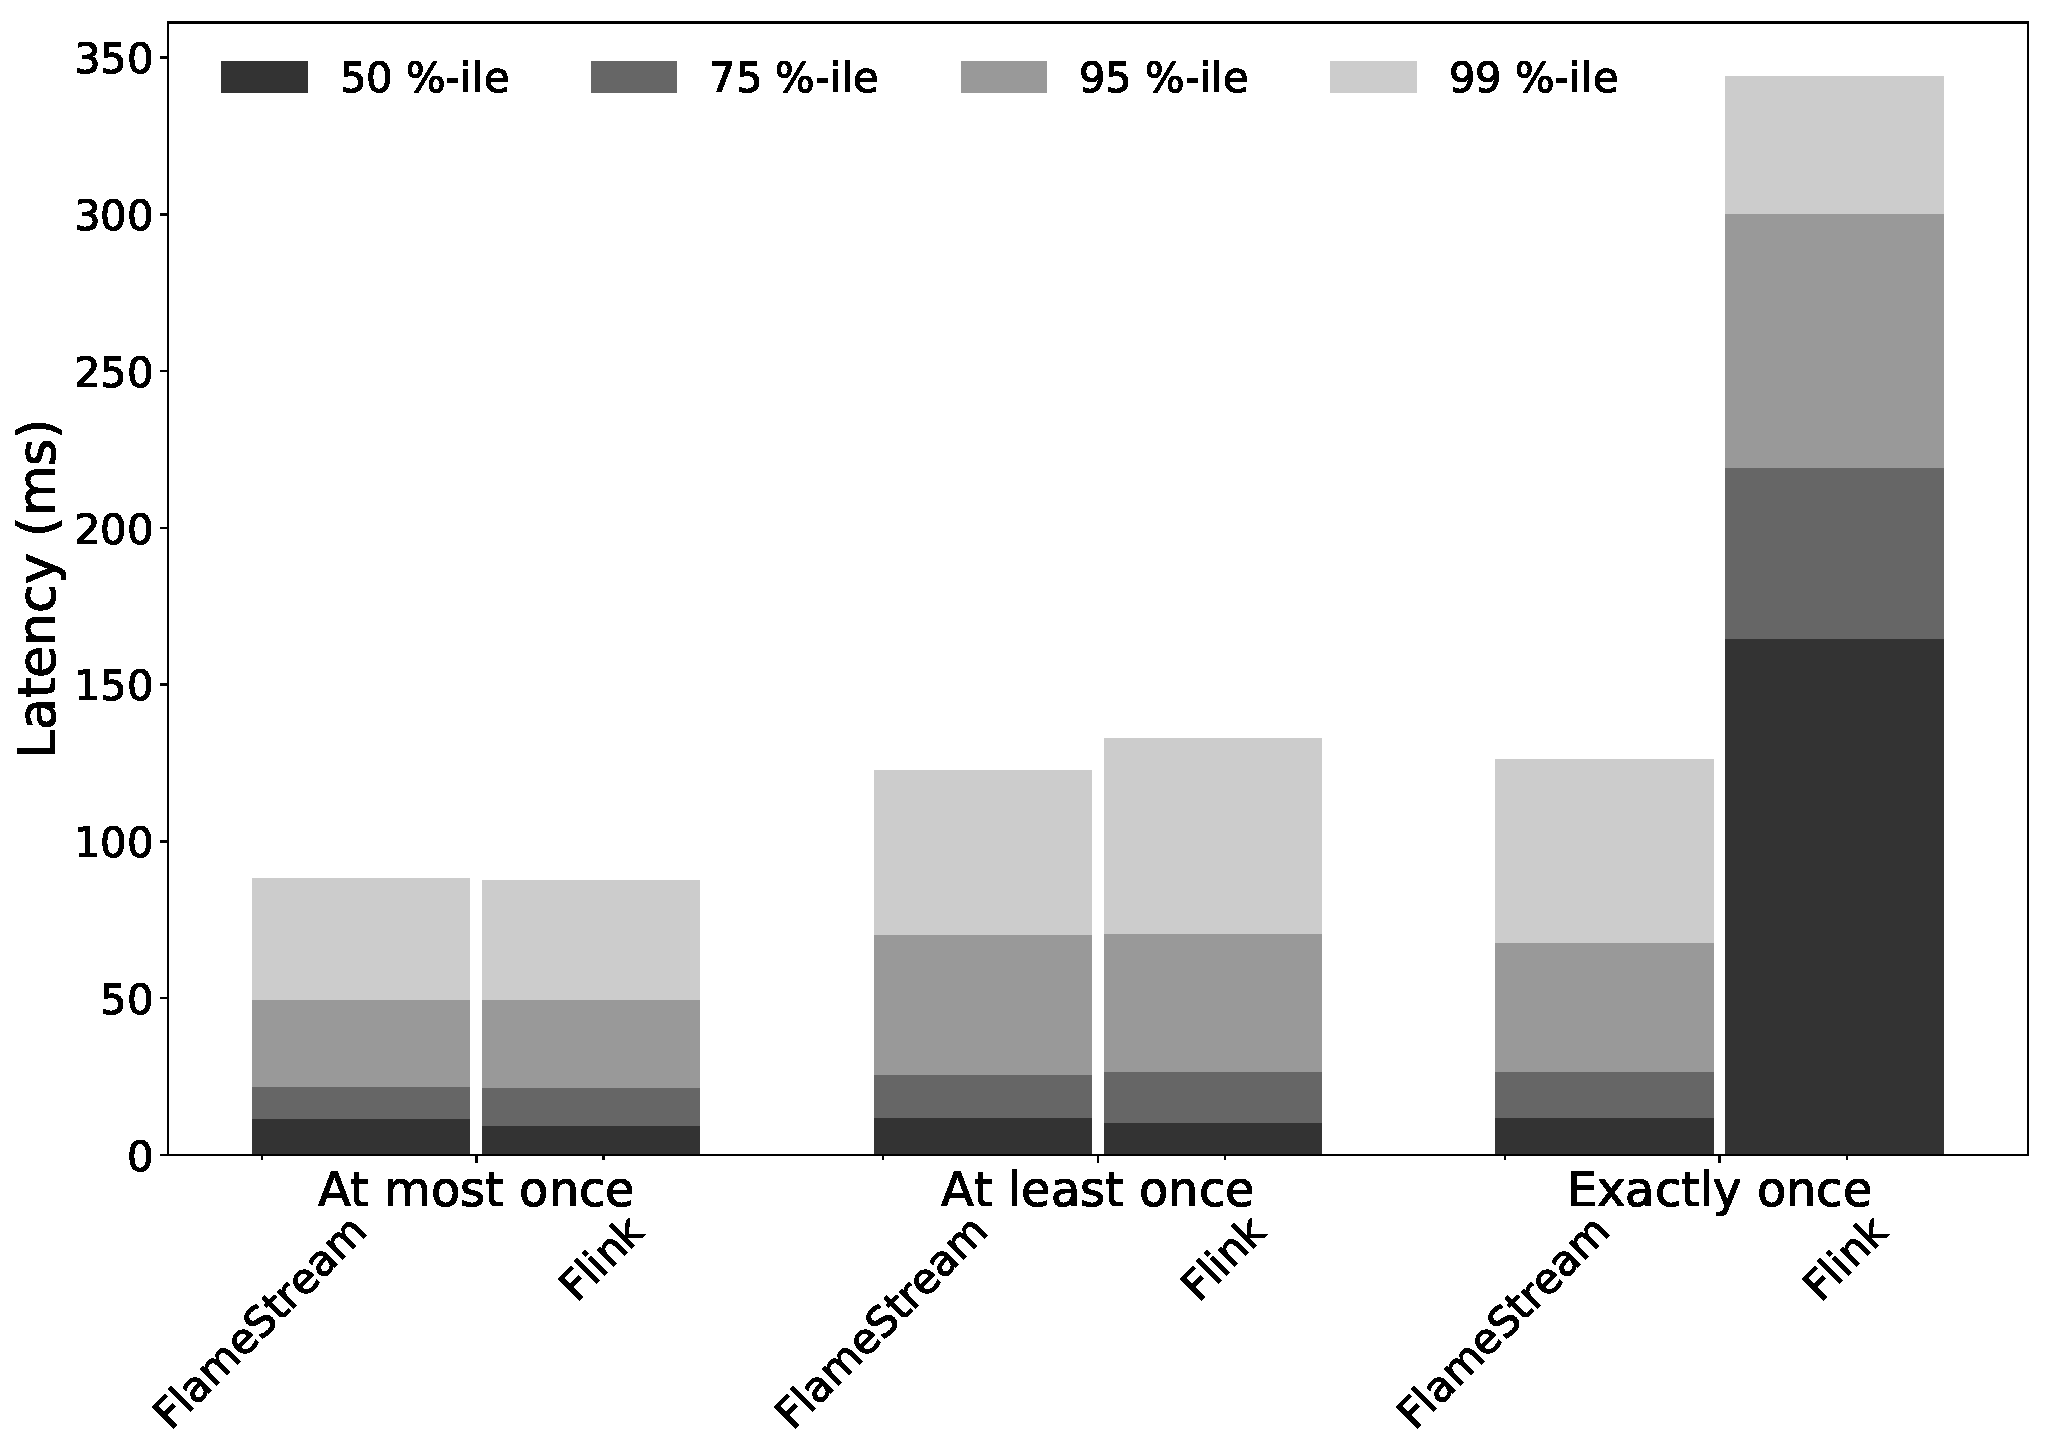
\includegraphics[width=.5\textwidth]{pics/comparison50}
  \caption{The comparison in latencies between \FlameStream\ and Flink with 50 ms delay between checkpoints}
  \label {comparison50}
\end{figure}

\begin{figure}[htbp]
  \centering
  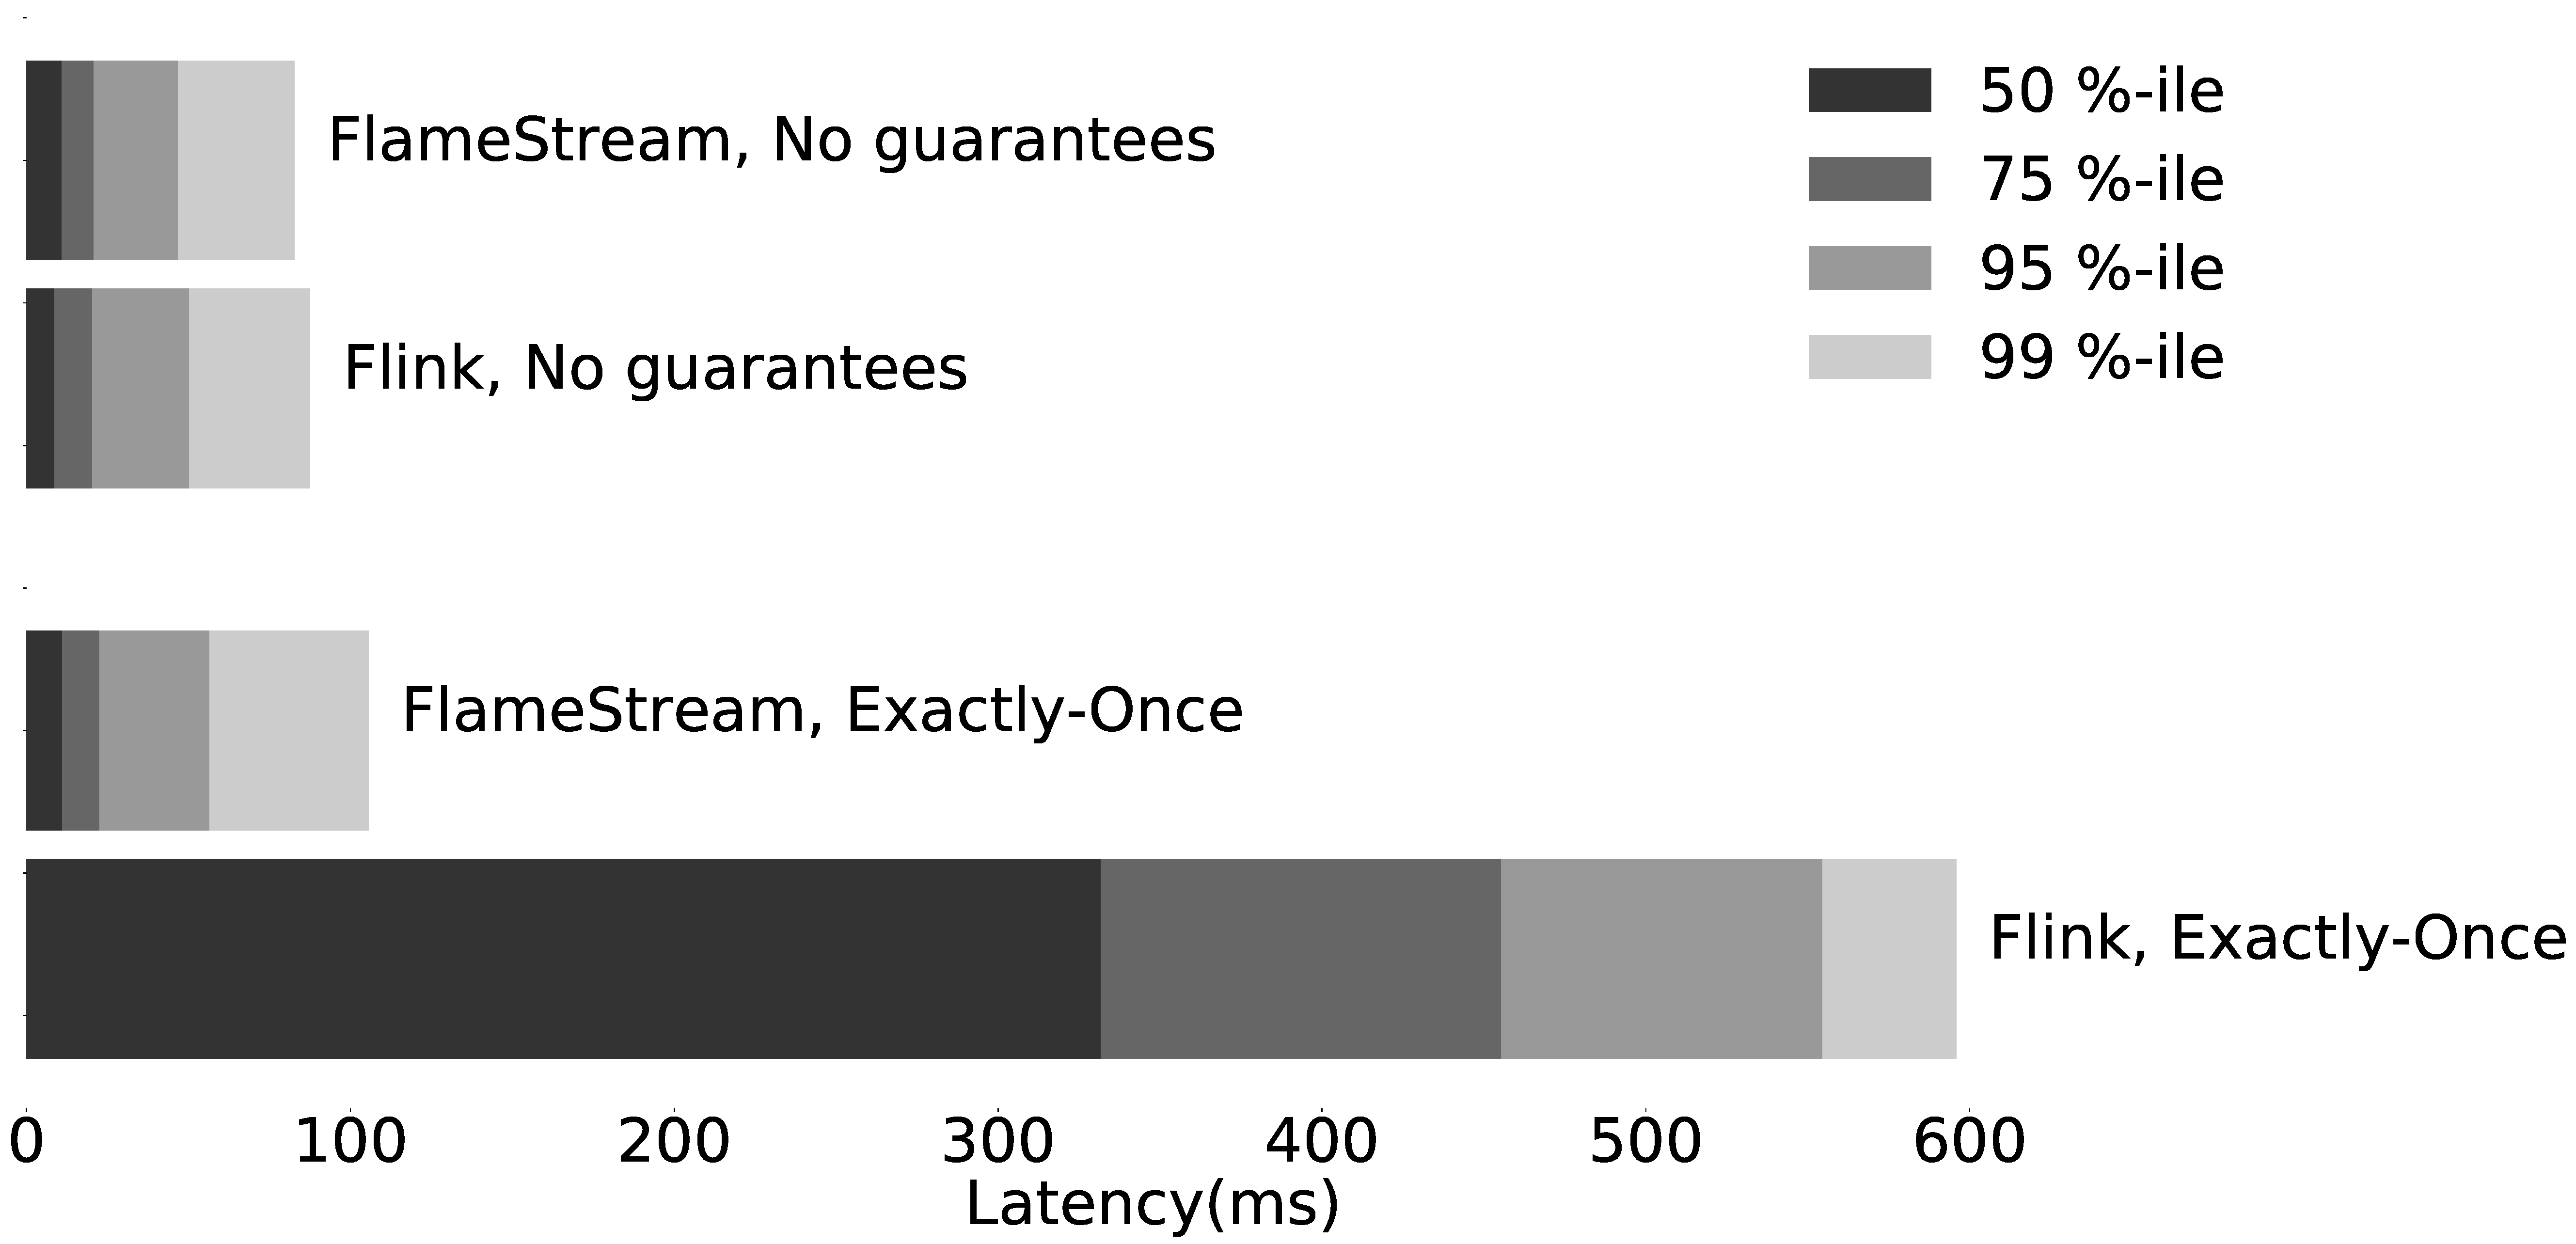
\includegraphics[width=.5\textwidth]{pics/comparison500}
  \caption{The comparison in latencies between \FlameStream\ and Flink with 500 ms delay between checkpoints}
  \label {comparison500}
\end{figure}

\begin{figure}[htbp]
  \centering
  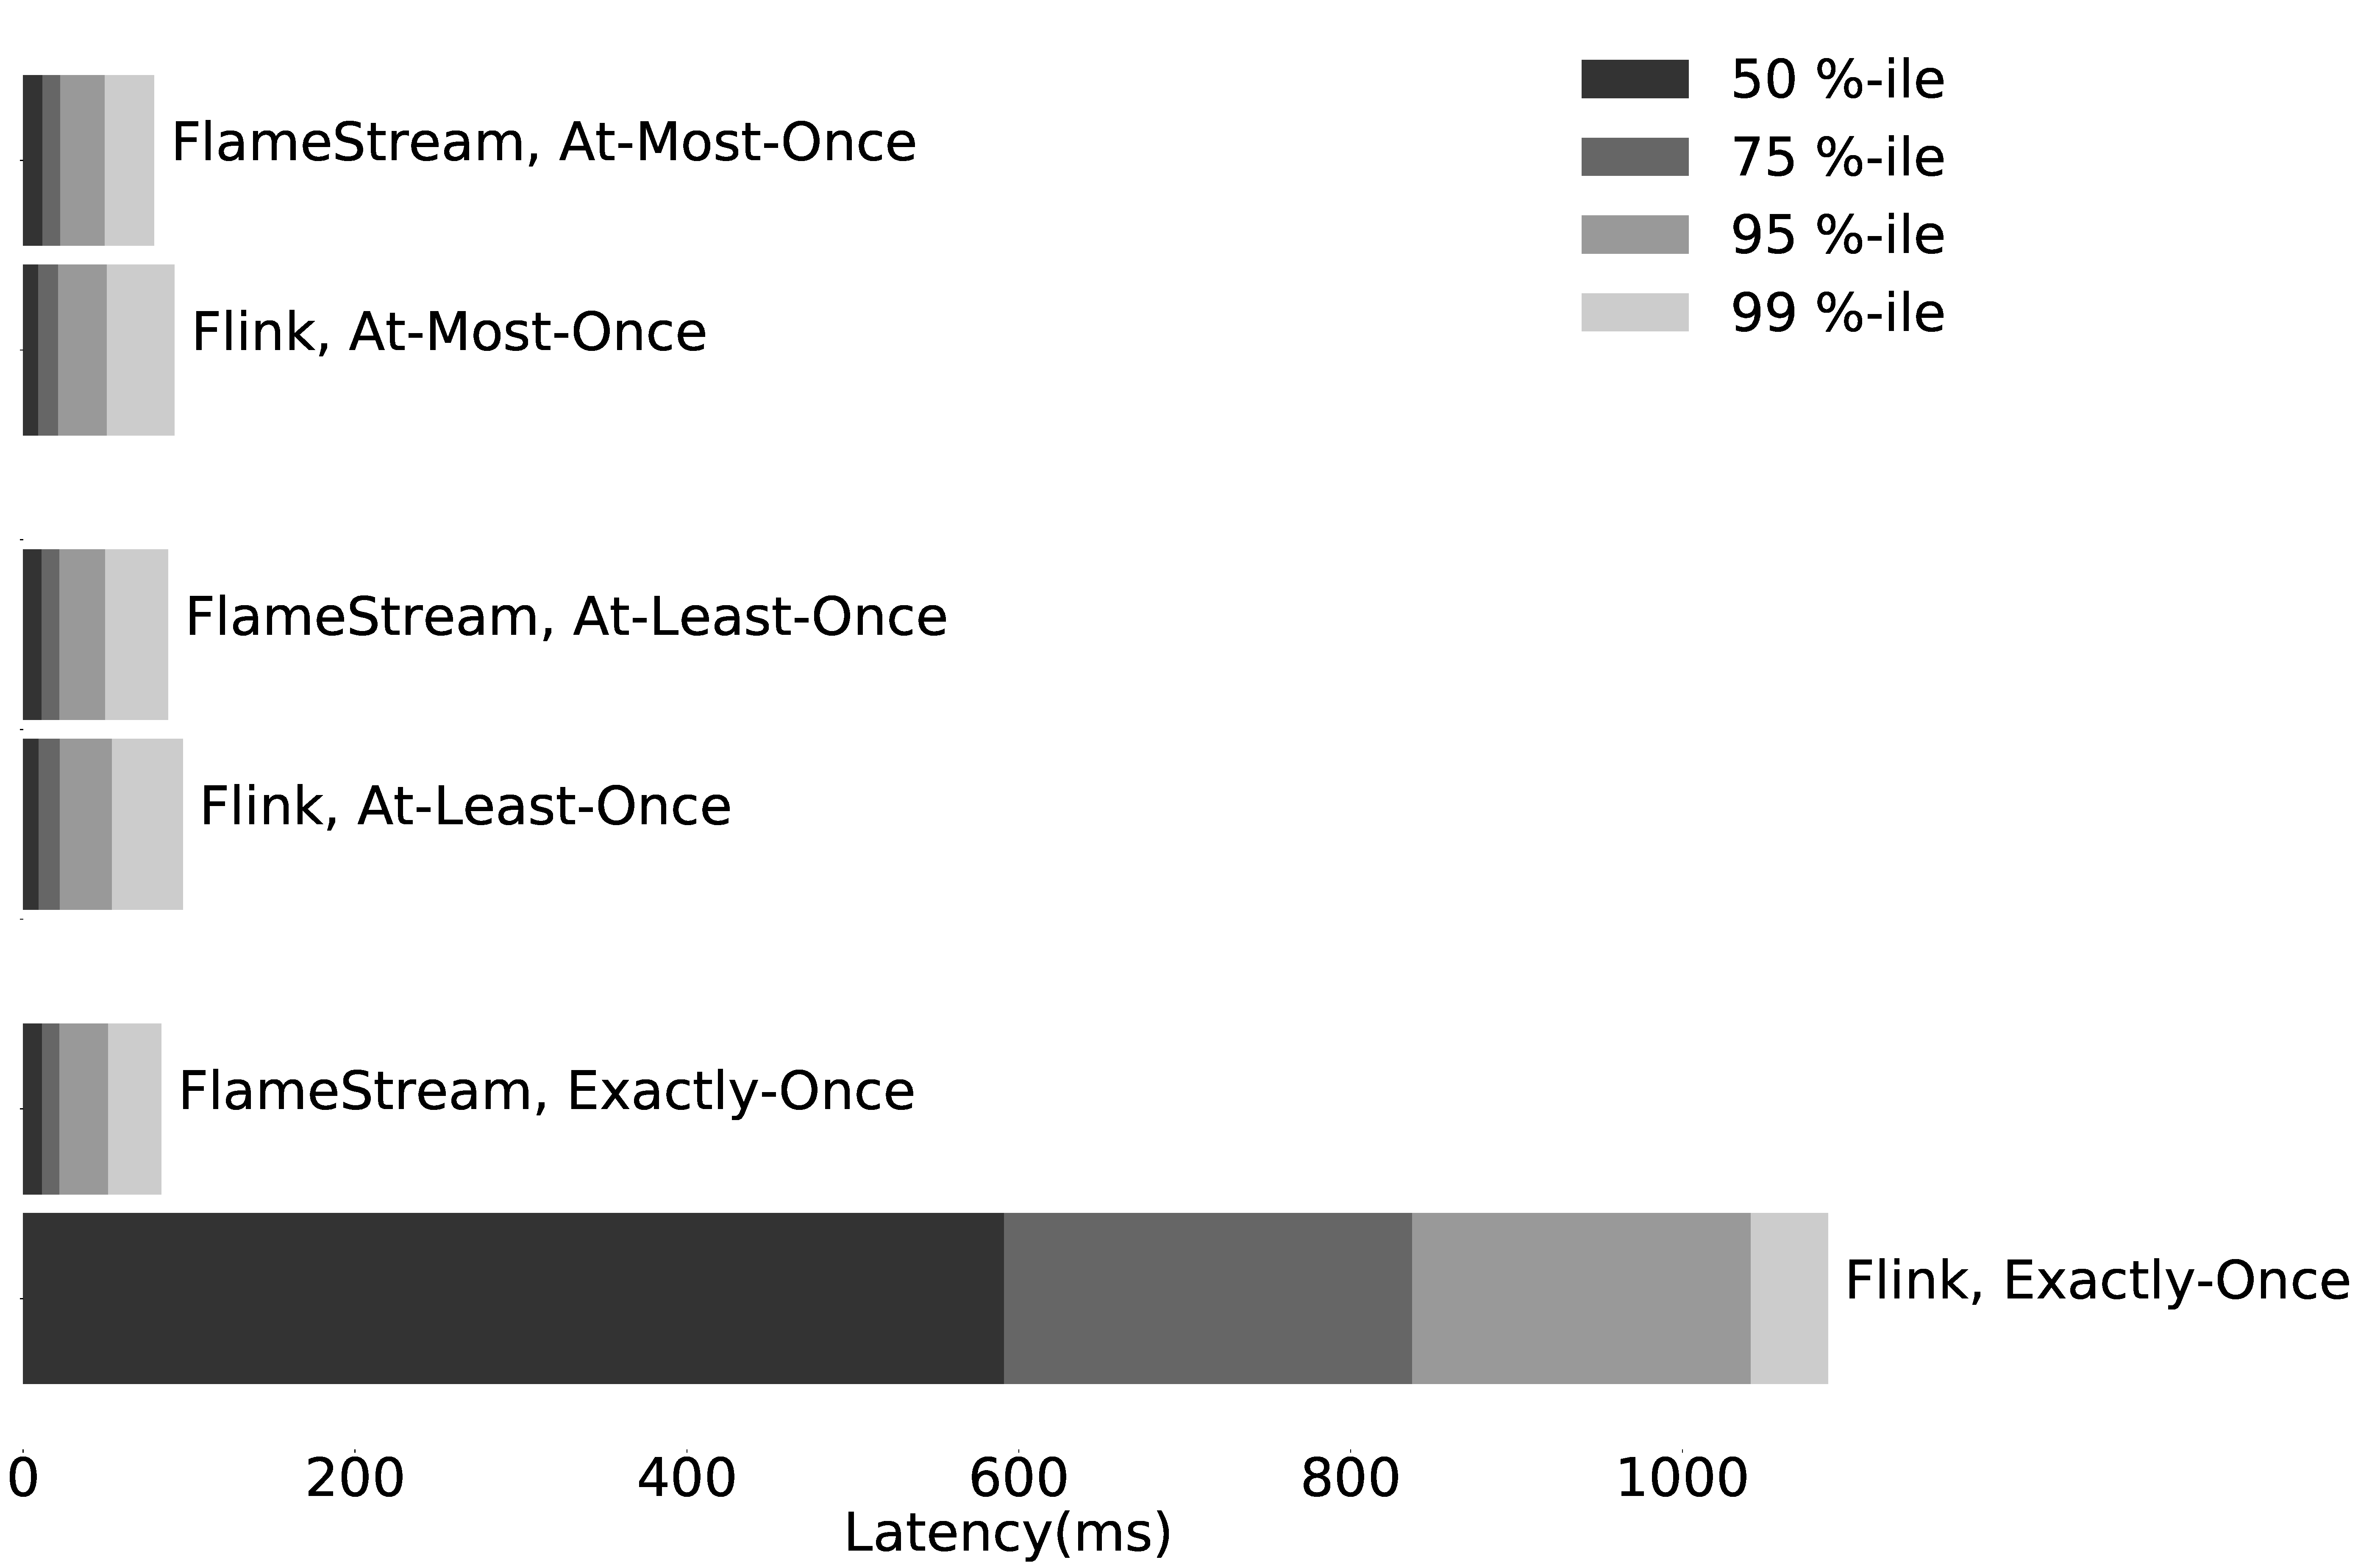
\includegraphics[width=.5\textwidth]{pics/comparison1000}
  \caption{The comparison in latencies between \FlameStream\ and Flink with 1000 ms delay between checkpoints}
  \label {comparison1000}
\end{figure}


\section {Related work}
%%% fs-state-related - Related work

\label {fs-related-seciton}

Techniques for providing exactly once are mentioned in details in section~\ref{fs-intro-seciton}. This topic is investigated in~\cite{Carbone:2017:SMA:3137765.3137777, Akidau:2013:MFS:2536222.2536229, Zaharia:2012:DSE:2342763.2342773}. Many prior works in the field of stream processing do not consider exactly once maintenance. For instance, Aurora~\cite{Abadi:2003:ANM:950481.950485} and Borealis~\cite{abadi2005design} do not provide any guarantees on data at all. Some other works provide only partial consistency. Apache Storm~\cite{apache:storm} supports message tracking mechanism that prevents the loss of data. However, exactly-once semantics is not provided, because duplicates are still possible. Twitter Heron, that was presented as the next generation of Apache Storm~\cite{Kulkarni:2015:THS:2723372.2742788}, does not provide for exactly-once as well. Samza~\cite{Noghabi:2017:SSS:3137765.3137770} also implements fairly similar to Storm model and has the same consistency guarantees.

Prior works on stream processing formalization concentrate on operations specification rather than delivery guarantees. Logical foundation for specifying streaming computations is discussed in~\cite{alur2018interfaces}. Declarative algebraic notations for the streaming queries are introduced in~\cite{halle2014formalization}. Another direction in streaming formalization is designing frameworks to define operations semantics~\cite{beck2018lars}.

\section {Conclusion and future work}
%%% fs-state-conclusion - Conclusion

\label {fs-conclusion-seciton}

We recognized that the lack of determinism in state-of-the-art stream processing systems makes consistency guarantees extremely hard to provide without the heavy overhead. Most of the systems use one of the following approaches: 
\begin{itemize}
    \item Enforcing determinism by micro-batching or buffering before each stateful operation
    \item Applying protocols that connect state snapshotting and data releasing in a transactional fashion
\end{itemize}

As it was shown, both methods are not suitable for latency-sensitive tasks. 

In this work, we introduced the deterministic model for distributed stream processing and demonstrated how properties of this model can be applied for providing strong consistency and fault tolerance. More precisely, we designed protocols, which allow to provide the following features:

\begin{itemize}
    \item The processes of business-logic computations, state snapshotting and releasing output items work asynchronously and independently
    \item At least once or exactly-once semantics is preserved even in the presence of failures
\end{itemize}

We implemented the prototype of the proposed model to examine its performance and scalability. Our experiments demonstrated that the introduced protocols for fault tolerance are scalable and provides remarkably low overhead within different computational layouts. Furthermore, the comparison with industrial stream processing solution indicated that our prototype can provide significantly lower latency.

Regarding future work, we plan to implement mechanisms for periodically rebuilding and redeploying execution graphs. This functionality can be used for graph generation based on some declarative language.

\balance

\bibliographystyle{abbrv}
\bibliography{../../bibliography/flame-stream}
\end {document}

\endinput
you can put whatever here

------------

reformulate in intro and preliminaries = one item enters, another leaves

защитить привязку или отвязку к Лампорту

убрать персистент

убрать рассуждение про полный реплей

в формализме прописать алгоритм рекавери

Внести рековери в определние снепшота или отдельное определение

явно сказать про распределенность в модели

сказать про граф в модели - D

сказать про консистентный снепшот в модели - Cl-1 и дырки

